%%%%%%%%%%%%%%%%%%%%%%%%%%%%%%%%%%%%%%%%%
% University/School Laboratory Report
% LaTeX Template
% Version 3.1 (25/3/14)
%
% This template has been downloaded from:
% http://www.LaTeXTemplates.com
%
% Original author:
% Linux and Unix Users Group at Virginia Tech Wiki 
% (https://vtluug.org/wiki/Example_LaTeX_chem_lab_report)
%
% License:
% CC BY-NC-SA 3.0 (http://creativecommons.org/licenses/by-nc-sa/3.0/)
%
% Modified by:
% Bartlomiej Dybisz
% Warsaw university of Technology
%
%%%%%%%%%%%%%%%%%%%%%%%%%%%%%%%%%%%%%%%%%

%----------------------------------------------------------------------------------------
%	PACKAGES AND DOCUMENT CONFIGURATIONS
%----------------------------------------------------------------------------------------

\documentclass{article}

\usepackage[version=3]{mhchem} % Package for chemical equation typesetting
\usepackage{siunitx} % Provides the \SI{}{} and \si{} command for typesetting SI units
\usepackage{graphicx} % Required for the inclusion of images
\usepackage{amsmath} % Required for some math elements 
\usepackage{url} % for bibliograpy links
\usepackage{float} % To force image to stand still
\usepackage[export]{adjustbox}
\usepackage[usenames, dvipsnames]{color} % to color some important remarks
\usepackage{caption}
\usepackage{subcaption}
\urlstyle{same}  % (for bibliography links
\setlength\parindent{0pt} % Removes all indentation from paragraphs

\renewcommand{\labelenumi}{\alph{enumi}.} % Make numbering in the enumerate environment by letter rather than number (e.g. section 6)

%\usepackage{times} % Uncomment to use the Times New Roman font

%----------------------------------------------------------------------------------------
%	DOCUMENT INFORMATION
%----------------------------------------------------------------------------------------

\title{Analysis and Processing of Biometric Images \\ Laboratory 3} % Title

\author{Bartłomiej \textsc{Dybisz}} % Author name

\date{\today} % Date for the report

\begin{document}

\maketitle % Insert the title, author and date

\begin{center}
\begin{tabular}{l r}
Date Performed: & October 31 , 2015 \\ % Date the experiment was performed
Instructor: & mgr Piotr Panasiuk % Instructor/supervisor
\end{tabular}
\end{center}

% If you wish to include an abstract, uncomment the lines below
% \begin{abstract}
% Abstract text
% \end{abstract}

%----------------------------------------------------------------------------------------
%	SECTION 1
%----------------------------------------------------------------------------------------

\section{Objectives}

% If you have more than one objective, uncomment the below:
\begin{description}
\item[Tresholding] \hfill \\
To learn how to implement tresholding - in particular binarization. In addition, to see how it affects processed image.
\item[Histogram Normalization] \hfill \\
To learn how to implement two approaches of histogram normalization and to determine differences between output images.
\item[Brightness] \hfill \\
To learn how to implement brightness control over pixels of an image. 
\end{description}

\subsection{Definitions}
\label{definitions}
\textcolor{red}{Remark:} throughout this report I will assume that each of red, green, blue channels of a pixel can take values from $0$ to $1$. It is imposed by JavaFX 8 - technology used to implement algorithms.

\begin{description}
\item[Tresholding]
A process of creating a black-and-white image out of a grayscale image consisting of setting exactly those pixels to white whose value is above a given threshold, setting the other pixels to black \cite{tresholding_def}.
\item[Image Histogram]
An image histogram is a graphical representation of the number of pixels in an image as a function of their intensity.
Histograms are made up of bins, each bin representing a certain intensity value range. The histogram is computed by examining all pixels in the image and assigning each to a bin depending on the pixel intensity. The final value of a bin is the number of pixels assigned to it. The number of bins in which the whole intensity range is divided is usually in the order of the square root of the number of pixels \cite{image_histogram_def}.
\item[Histogram Normalization]
In image processing, normalization is a process that changes the range of pixel intensity values. Applications include photographs with poor contrast due to glare, for example. Normalization is sometimes called contrast stretching or histogram stretching \cite{histogram_normalization_def}. 

As one can find in literature, general equation for this process is as follows:
\[
(\forall{p \in pixels} )(I(p) = (I(p) - minPix) * \frac{intMax - intMin}{maxPix - minPix} + intMin)
\]
, where $intMax$ and $intMin$ correspond to the limits over which image intensity values will be extended,
$minPix$ and $maxPix$ are values of minimal and maximal saturation of image's pixels and $I(p)$ defines intensity of pixel $p$.

However, since we discuss only standard 8-bit grayscale images, values will be stretched over $\langle0;1\rangle$ interval (as mentioned in remark to this section), hence $intMax = 1$ and $intMin = 0$, which will cause above equation to look as:
\begin{equation} \label{eq:1}
(\forall{p \in pixels} )(I(p) = (I(p) - minPix) * \frac{1}{maxPix - minPix})
\end{equation}

In our experiment we assumed that input picture is not grayscale, hence it is not true that for every channel saturation of red, green and blue channels must be the same. In consequence, we apply equation \ref{eq:1} to each channel separately. In addition, two approaches were adopt;
\begin{itemize}
  \item $maxPix$ and $minPix$ were chosen for each channel separately (i.e. applying \ref{eq:1} to channel red, we consider minimum and maximum saturation of red channel of the whole image. Similarly for green and blue channel).
  \item $maxPix$ and $minPix$ were calculated as an average of minimal and maximal values of all three channels.
\end{itemize}

\item[Brightness]
Image brightness (or luminous brightness) is a measure of intensity after the image has been acquired with a digital camera or digitized by an analog-to-digital converter\cite{{brightness_def1}}. 
\item[Brightness Manipulation]
We think of brightness manipulation as an increasing or decreasing intensity of each pixel. To express this we used following formula:
\begin{equation} \label{eq:2}
(\forall{p \in pixels} )(I(p) = I(p) + brigthness)
\end{equation}
It is important to remember about clamping values of all pixels between $0$ and $1$ (convention assumed in remark to this section).

\end{description} 

 
%----------------------------------------------------------------------------------------
%	SECTION 2
%----------------------------------------------------------------------------------------

\section{Experimental Data}
Since laboratory concerned processing of images, it is not a surprise that our data were images. Although during session we check algorithms only for one picture, I'll demonstrate results on 3 additional ones to enrich this report. 

\begin{figure}[H]
\centering
\begin{subfigure}{.5\textwidth}
  \centering
  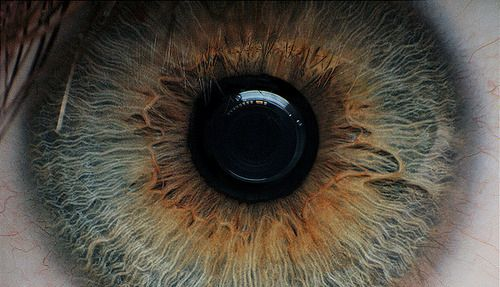
\includegraphics[width=0.97\linewidth]{_Figures/sample_1.jpg}
  \caption{}
  \label{fig:sample_1}
\end{subfigure}%
\begin{subfigure}{.5\textwidth}
  \centering
  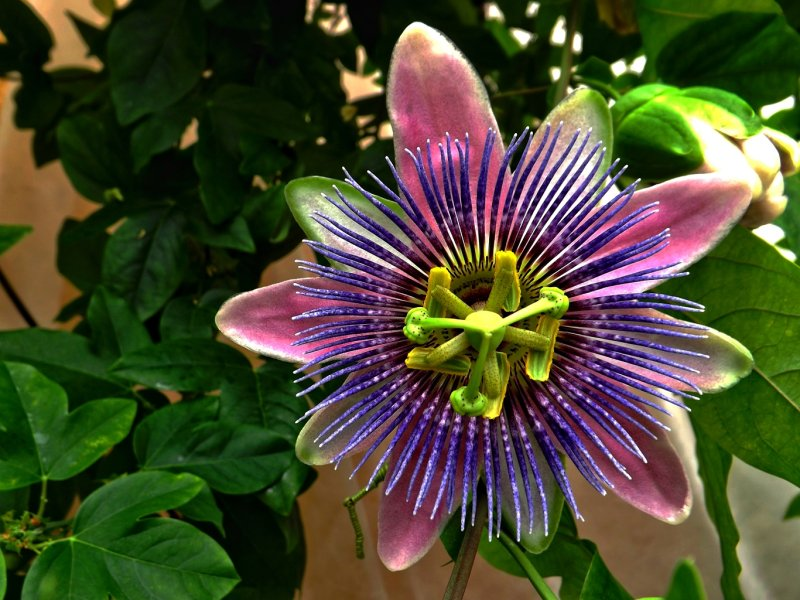
\includegraphics[width=0.97\linewidth]{_Figures/sample_2.jpg}
    \caption{}
  \label{fig:sample_2}
\end{subfigure}
\begin{subfigure}{.5\textwidth}
  \centering
  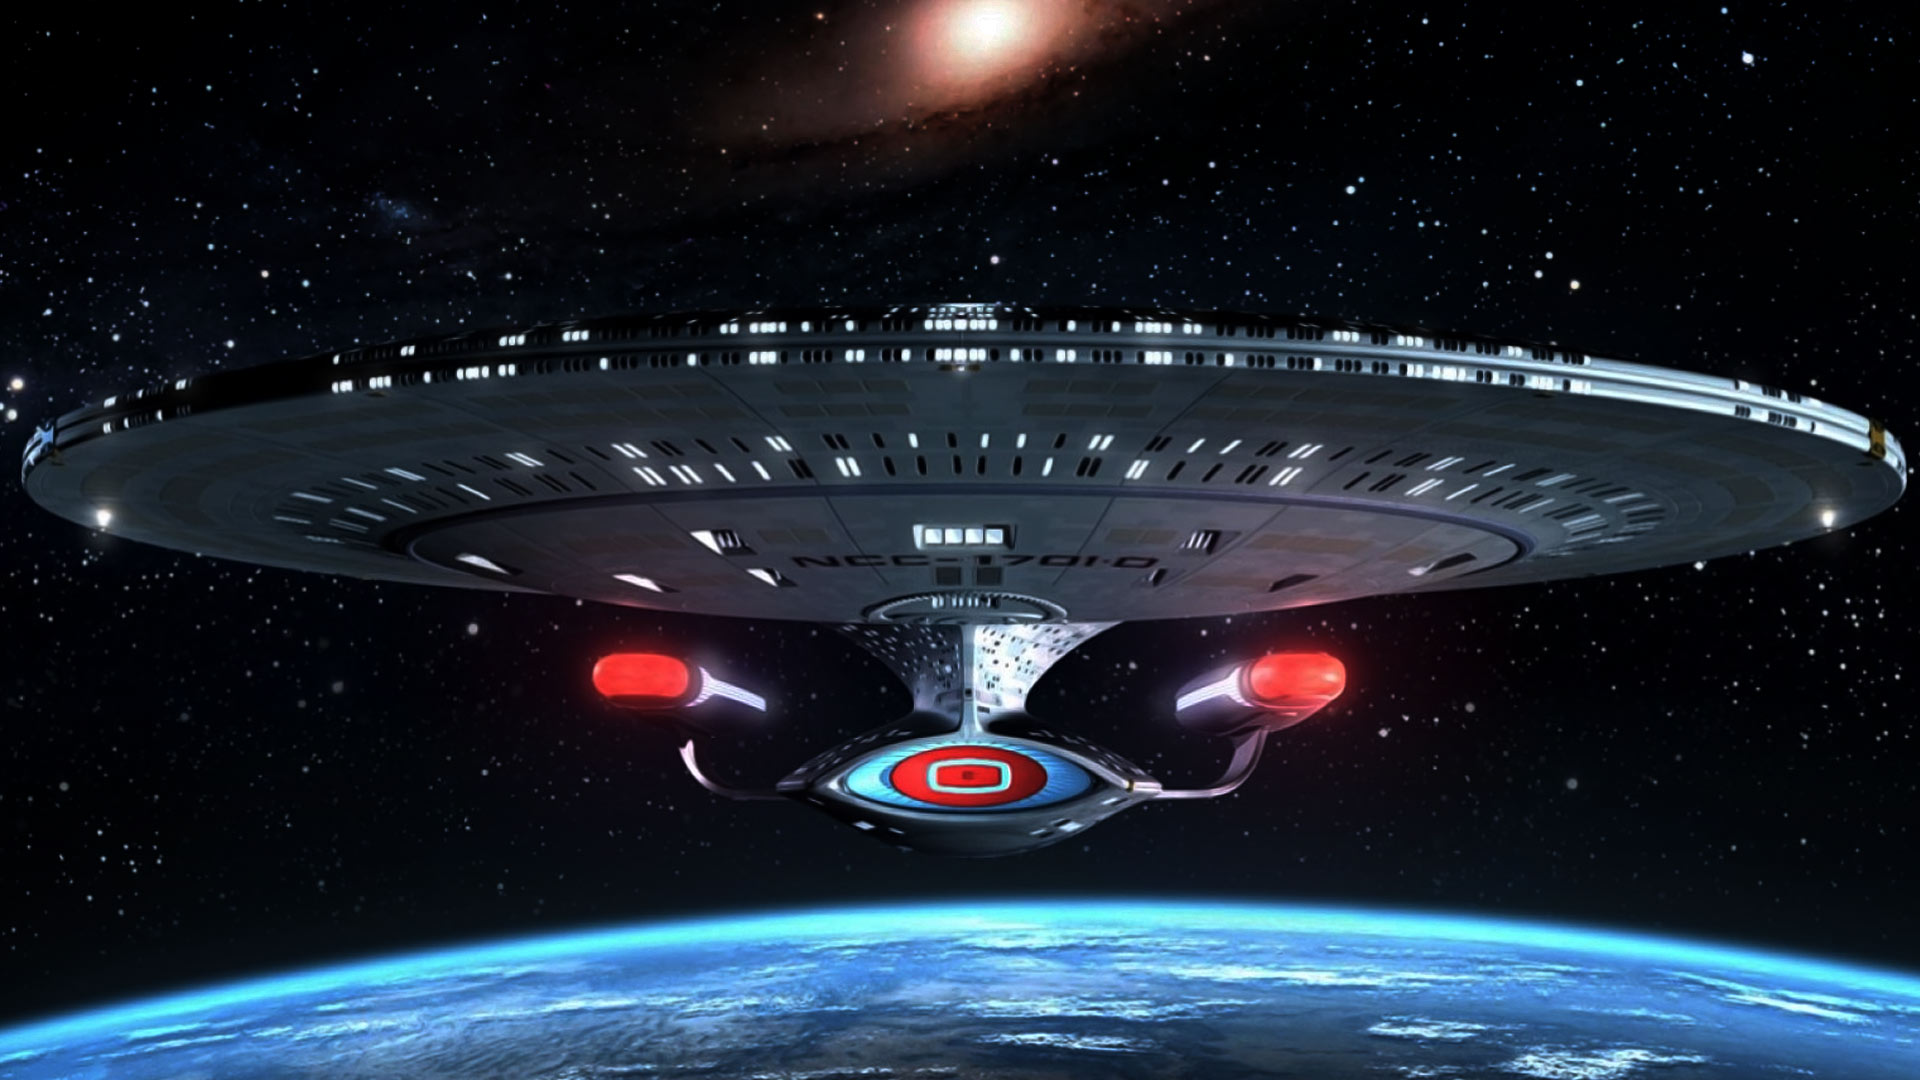
\includegraphics[width=0.97\linewidth]{_Figures/sample_3.jpg}
  \caption{}
  \label{fig:sample_3}
\end{subfigure}%
\begin{subfigure}{.5\textwidth}
  \centering
  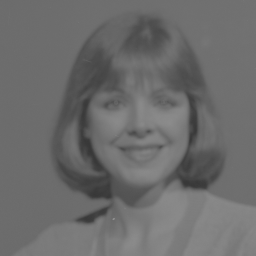
\includegraphics[width=0.97\linewidth]{_Figures/sample_4.png}
    \caption{}
  \label{fig:sample_4}
\end{subfigure}
\caption{Images used to check implemented algorithms.}
\label{fig:double_samples}
\end{figure}



%----------------------------------------------------------------------------------------
%	SECTION 3
%----------------------------------------------------------------------------------------

\newpage
\section{Sample Code}
This section contains code snippets with algorithms implementation. Each figures is provided with appropriate description either in caption or in method's comment. 

%
% CLASS DIAGRAM
%
\subsection{Operations Class Diagram}
Classes performing operations (tresholding, histogram normalization and brightness manipulation) inherit from Filter class. Such approach has been pursued because it may happen in future that polimorphism will be useful with e.g. dealing with list of filters, which should be applied to one image. Figure \ref{fig:class_diag} depicts dependencies.

\begin{figure}[H]
	\centering
	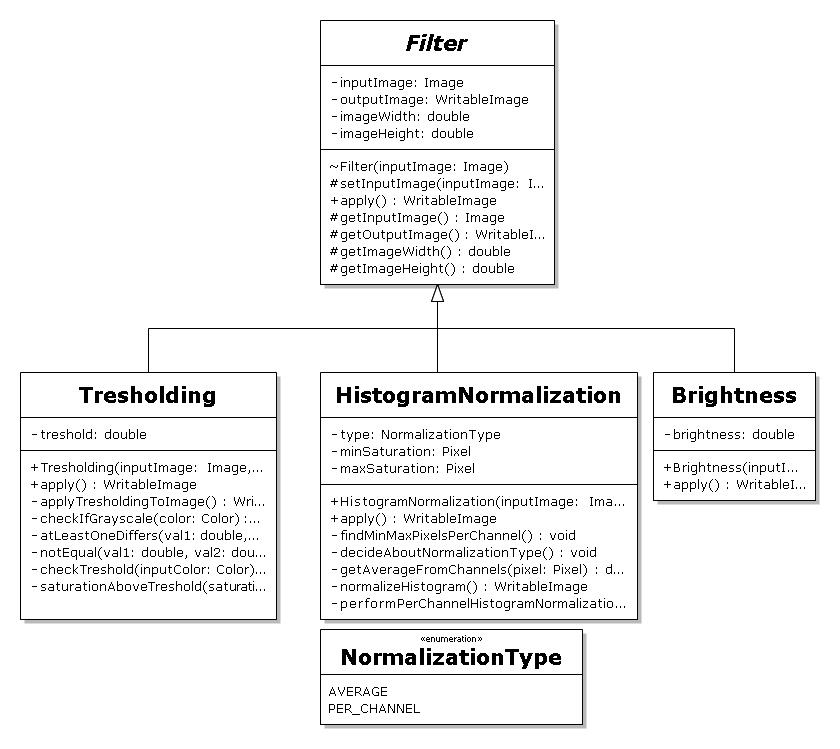
\includegraphics[width=0.9\textwidth]{_Figures/class_diagram_2.png}
    \caption{Class diagram of implemented operations.}
    \label{fig:class_diag}
\end{figure}

%
% TRESHOLDING IMPLEMENTATION
%
\subsection{Tresholding Implementation}

\begin{figure}[H]
	\centering
	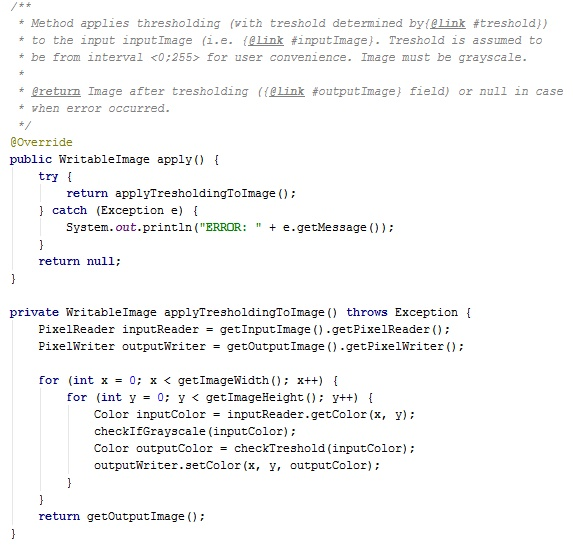
\includegraphics[width=0.95\textwidth]{_Figures/treshold_function.jpg}
    \caption{Overview of high abstraction level methods for tresholding. As one can see it may happens that input image is not in grayscale, in such a case appropriate exception is thrown (see figure \ref{fig:not_grayscale}).}
    \label{fig:code:treshold_func}
\end{figure}

\begin{figure}[H]
	\centering
	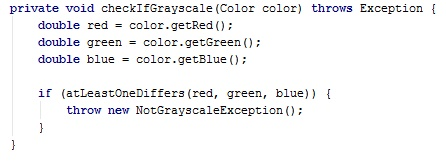
\includegraphics[width=0.7\textwidth, left]{_Figures/notGrayscale.jpg}
	\caption{Saturation on all channels is checked for equality.}
	\label{fig:not_grayscale}
\end{figure}
	
\begin{figure}[H]
	\centering
	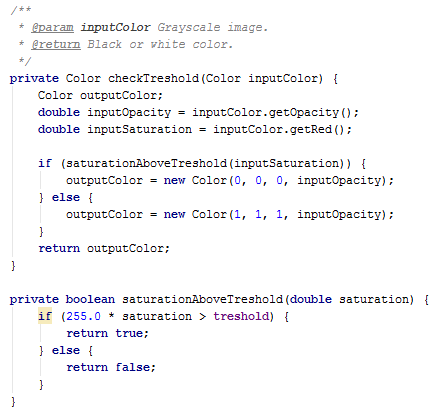
\includegraphics[width=0.7\textwidth]{_Figures/treshold_check.png}
	\caption{Here we can see one of the results of remark given to section \ref{definitions} - color saturation must be multiplied by 255.}
\end{figure}

%
% HISTOGRAM NORMALIZATION IMPLEMENTATION
%
\subsection{Histogram Normalization Implementation}

\begin{figure}[H]
	\centering
	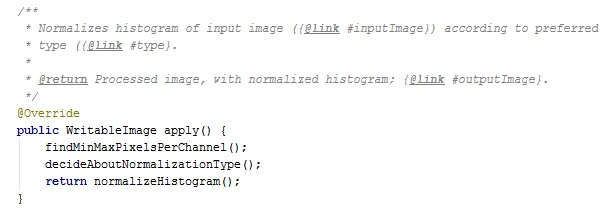
\includegraphics[width=0.95\textwidth]{_Figures/normalization_function.jpg}
	\caption{Main, highly abstract method applying histogram normalization.}
\end{figure}

\begin{figure}[H]
	\centering
	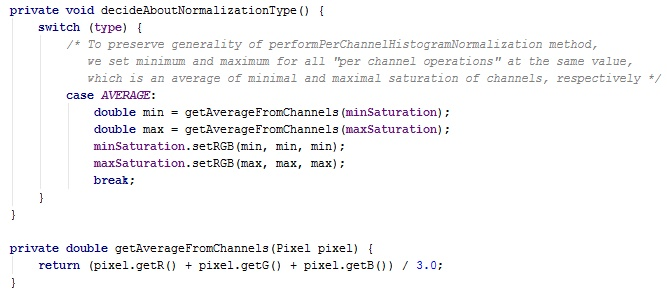
\includegraphics[width=0.95\textwidth]{_Figures/normalization_type.jpg}
\end{figure}

\begin{figure}[H]
	\centering
	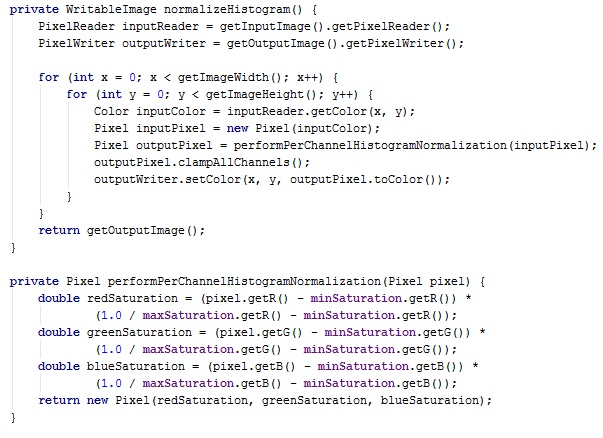
\includegraphics[width=1\textwidth]{_Figures/normalization_process.jpg}
	\caption{Lower abstraction shows more about implementation and presents equations from section \ref{definitions}, concerning histogram normalization.}
\end{figure}

%
% Brightness Implementation
%
\subsection*{Brightness Manipulation Implementation}
\begin{figure}[H]
	\centering
	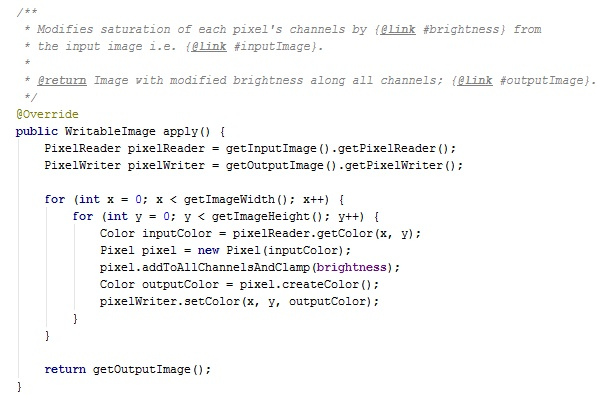
\includegraphics[width=1\textwidth]{_Figures/brigthness_function.jpg}
\end{figure}

\begin{figure}[H]
	\centering
	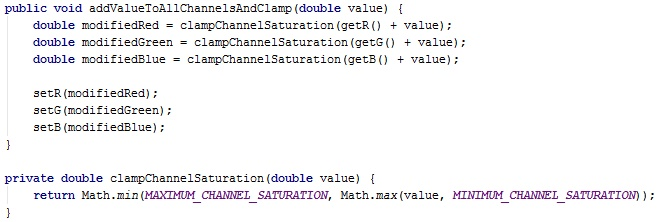
\includegraphics[width=1\textwidth]{_Figures/brighthness_clamp.jpg}
\end{figure}

%----------------------------------------------------------------------------------------
%	SECTION 4
%----------------------------------------------------------------------------------------

\section{Results and Conclusions}

%
% TRESHOLD
%
\subsection{Tresholding Results}
In case of tresholding, different pictures acts differently. To start with, figure \ref{fig:tresh_raw_1} acts greatly in case of iris extraction. As one can see image \ref{fig:tresh_good_1} presents extraction of  desired parts (treshold level 8). I have also notice that when treshold level is bigger than 40 (figure \ref{fig:tresh_bad_1}), image starts to have a lot of distortions in form of additional information about white of the eye.


On the other hand picture \ref{fig:tresh_raw_2} had rather average results comparing to all others. Although flower object can be distinguished from rest of the surrounding (treshold level 105) but there is always a significant amount of artifacts in background and elevating treshold (picture \ref{fig:tresh_bad_2}; level over 180) reveals only worse outcomes - flower borders are starting to disappear.

Figure \ref{fig:tresh_raw_3} behaves best in terms of tresholding. Distinguishing between a planet and USS Enterprise NCC-1701-D can be easily done at (treshold) level 32. Increasing treshold causes lost of information about ship along with background artifacts. I think that by finding good ratio between lost of the background noise and preserving Enterprise shape we will be able to still recreate the ship (e.g using dilatation filter) and clear the picture out of noise (to some reasonable level). Image \ref{fig:tresh_bad_3} presents treshold equal to 103.

Last one - figure \ref{fig:tresh_raw_1}, also reacts nicely to the tresholding process. At level 105 (\ref{fig:tresh_good_4}) it almost perfectly distinguish between hair and face, but slight changes to the treshold immediately causes lost of coherence, as can be seen on \ref{fig:tresh_bad_4}.



\begin{figure}[H]
\centering
\begin{subfigure}{.3\textwidth}
  \centering
  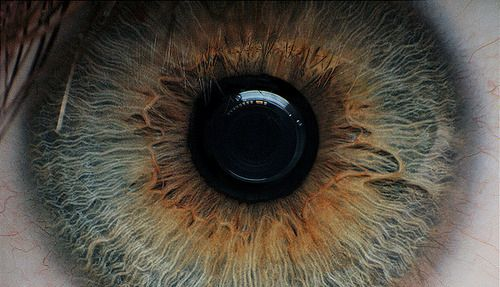
\includegraphics[width=0.97\linewidth]{_Figures/sample_1.jpg}
  \caption{}
  \label{fig:tresh_raw_1}
\end{subfigure}%
\begin{subfigure}{.3\textwidth}
  \centering
  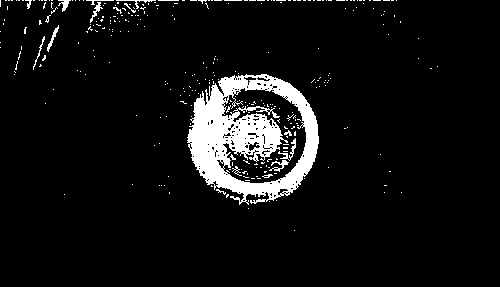
\includegraphics[width=0.97\linewidth]{_Figures/sample_1_good_treshold.png}
  \caption{}
  \label{fig:tresh_good_1}
\end{subfigure}%
\begin{subfigure}{.3\textwidth}
  \centering
  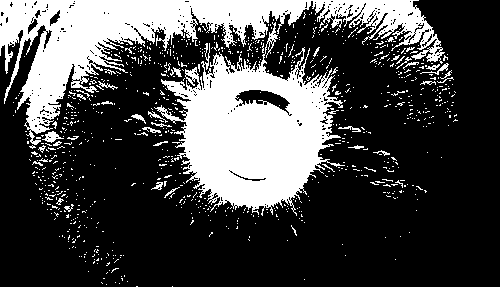
\includegraphics[width=0.97\linewidth]{_Figures/sample_1_bad_treshold.png}
    \caption{}
  \label{fig:tresh_bad_1}
\end{subfigure}

\begin{subfigure}{.3\textwidth}
  \centering
  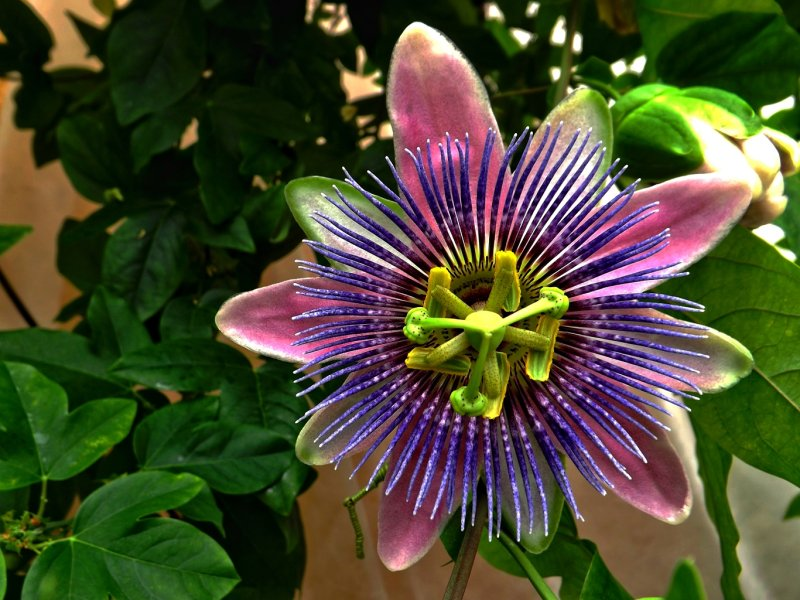
\includegraphics[width=0.97\linewidth]{_Figures/sample_2.jpg}
  \caption{}
  \label{fig:tresh_raw_2}
\end{subfigure}%
\begin{subfigure}{.3\textwidth}
  \centering
  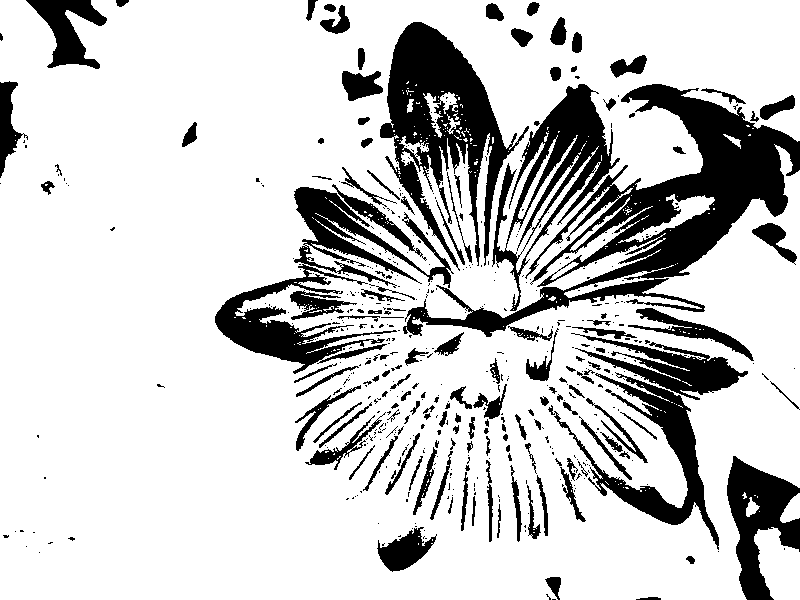
\includegraphics[width=0.97\linewidth]{_Figures/sample_2_good_treshold.png}
  \caption{}
  \label{fig:tresh_good_2}
\end{subfigure}%
\begin{subfigure}{.3\textwidth}
  \centering
  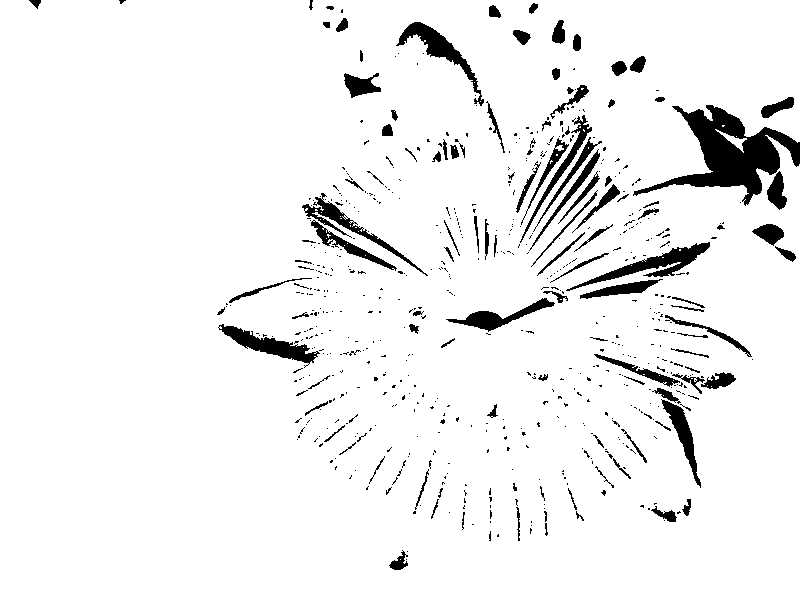
\includegraphics[width=0.97\linewidth]{_Figures/sample_2_bad_treshold.png}
    \caption{}
  \label{fig:tresh_bad_2}
\end{subfigure}

\begin{subfigure}{.3\textwidth}
  \centering
  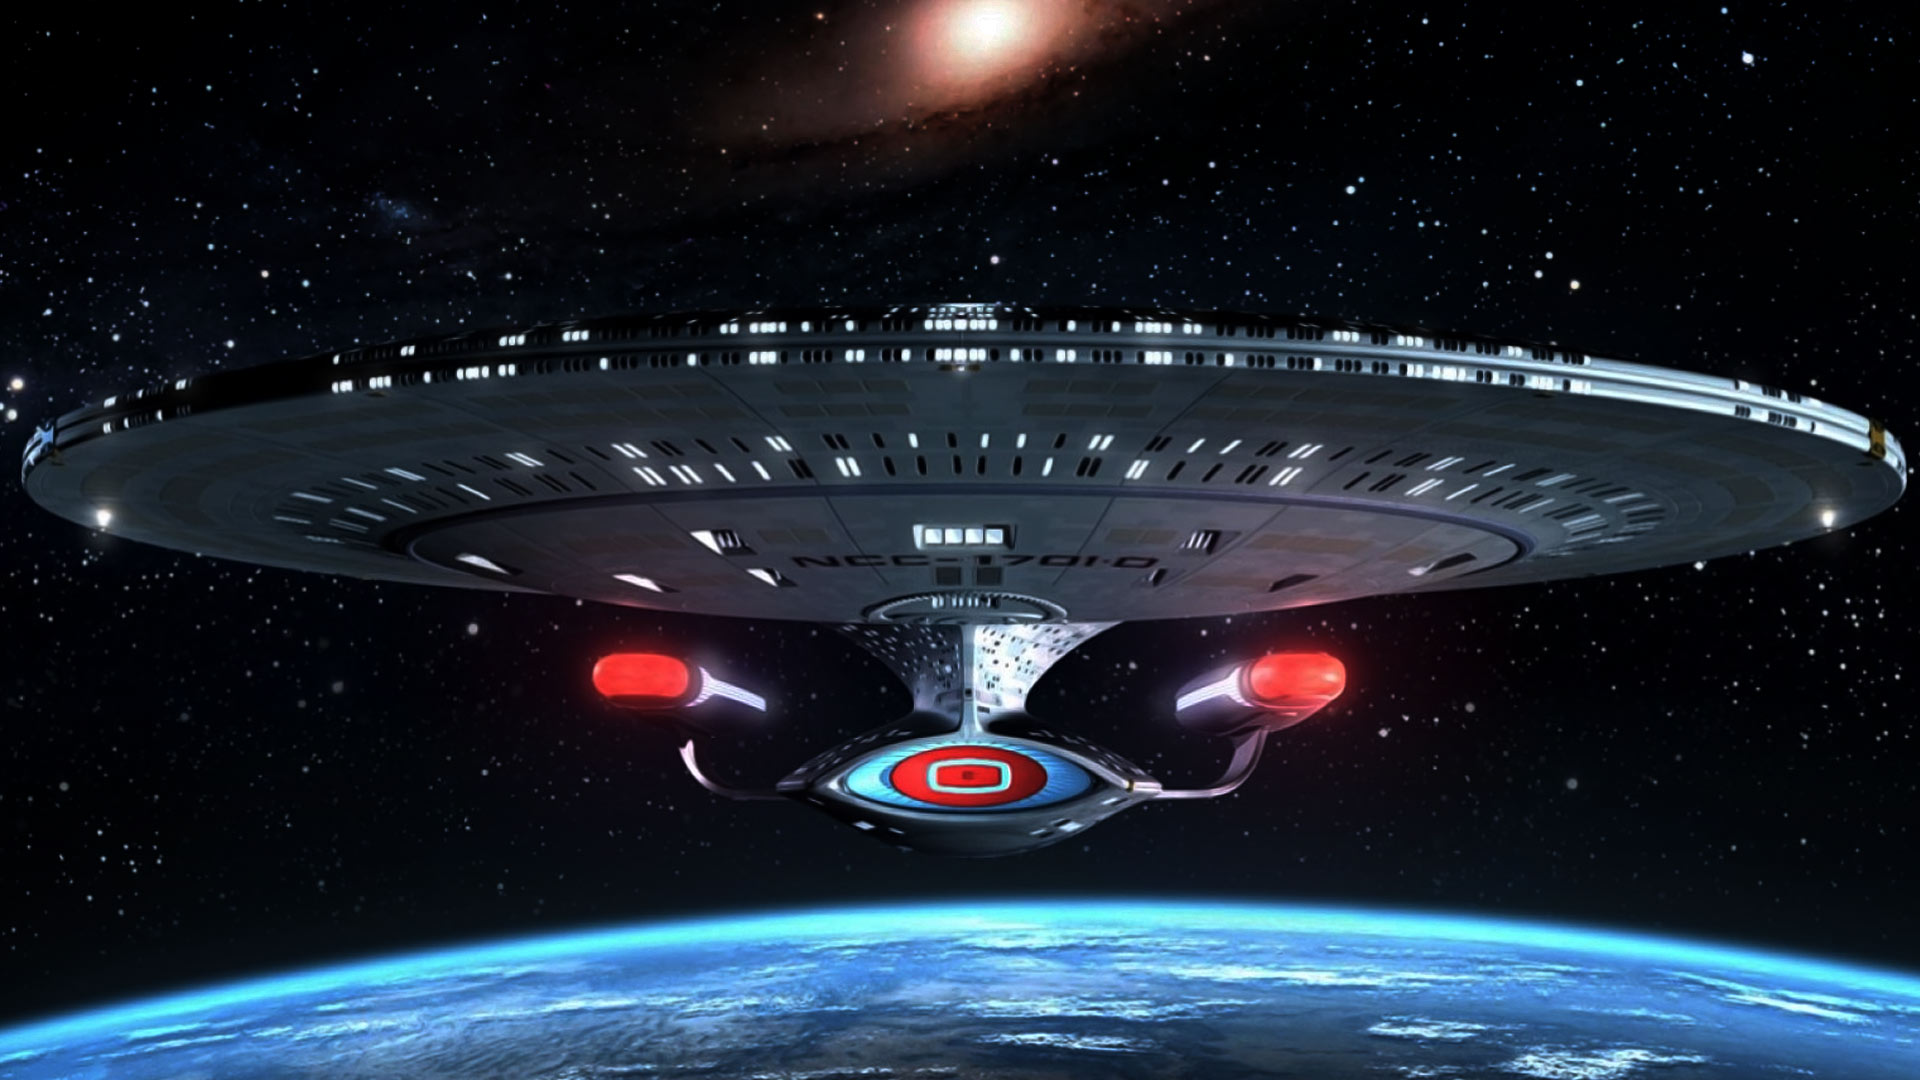
\includegraphics[width=0.97\linewidth]{_Figures/sample_3.jpg}
  \caption{}
  \label{fig:tresh_raw_3}
\end{subfigure}%
\begin{subfigure}{.3\textwidth}
  \centering
  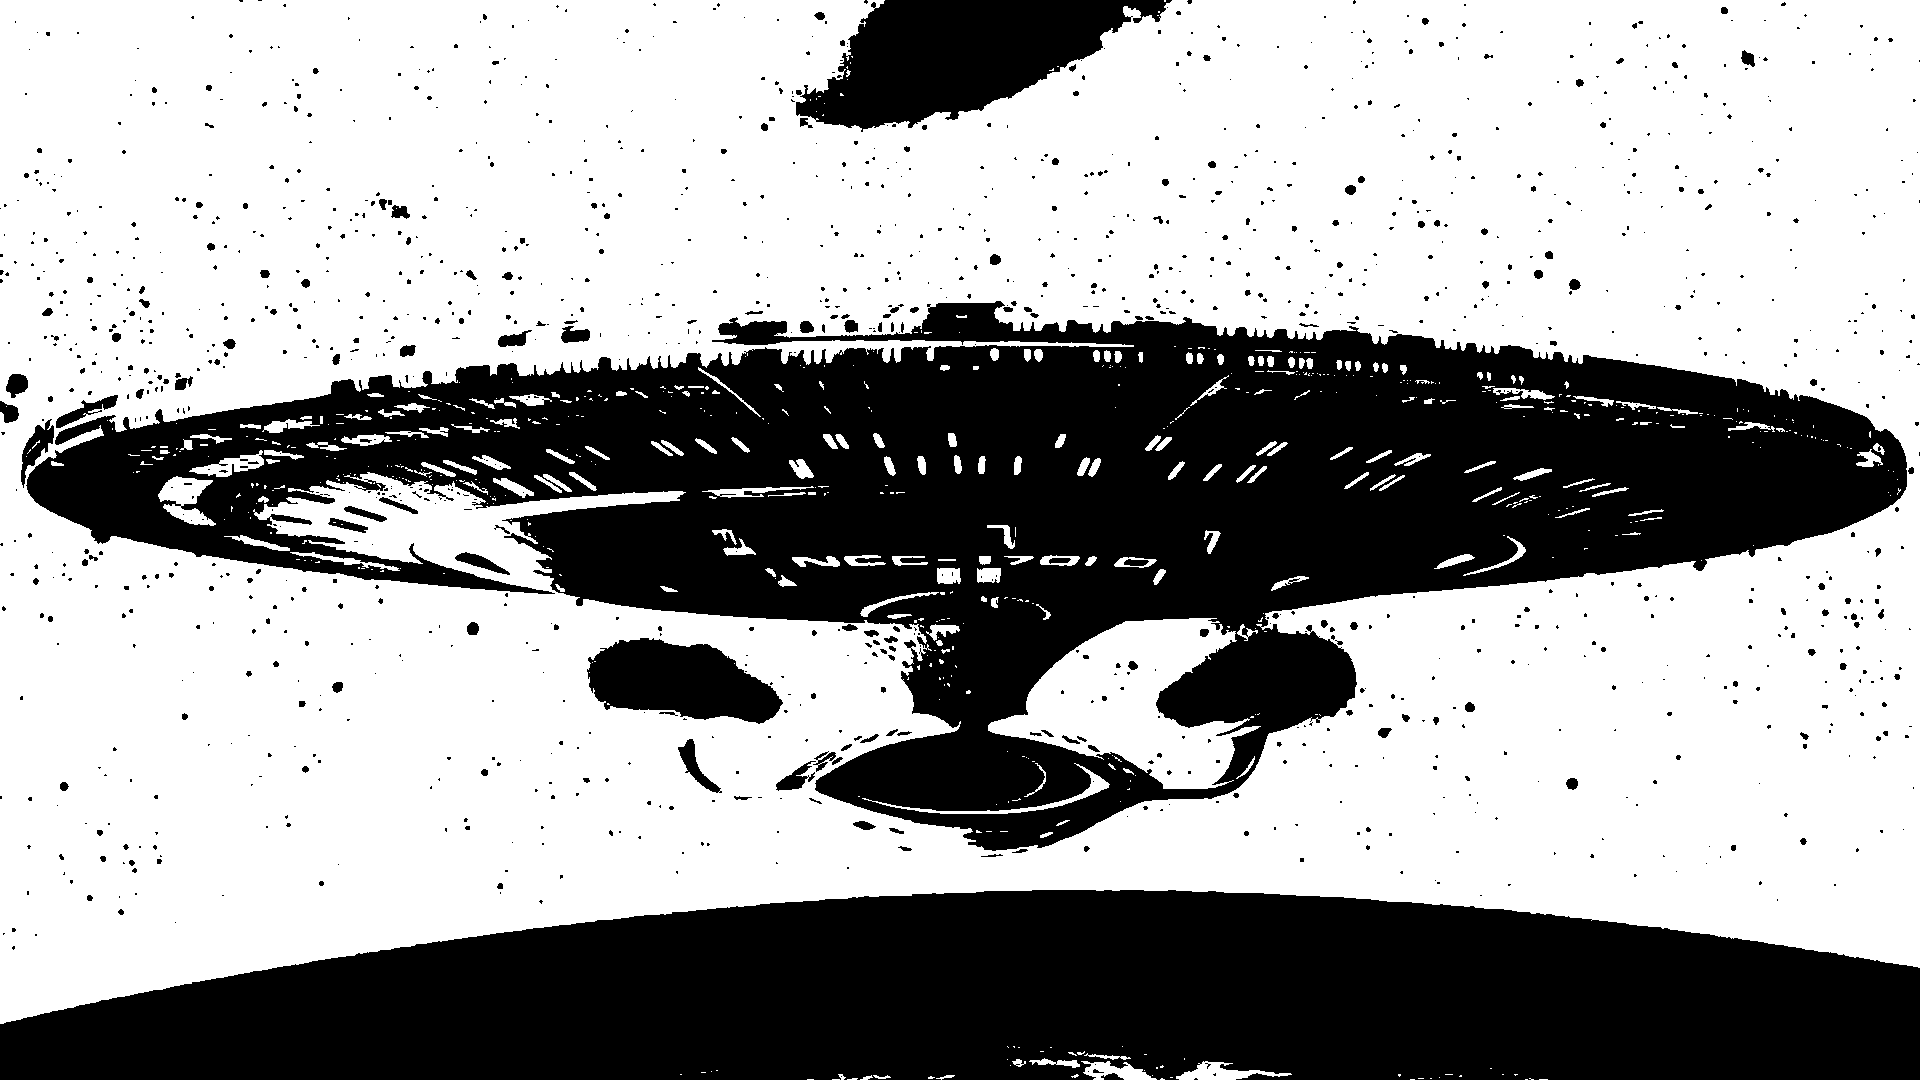
\includegraphics[width=0.97\linewidth]{_Figures/sample_3_good_treshold.png}
  \caption{}
  \label{fig:tresh_good_3}
\end{subfigure}%
\begin{subfigure}{.3\textwidth}
  \centering
  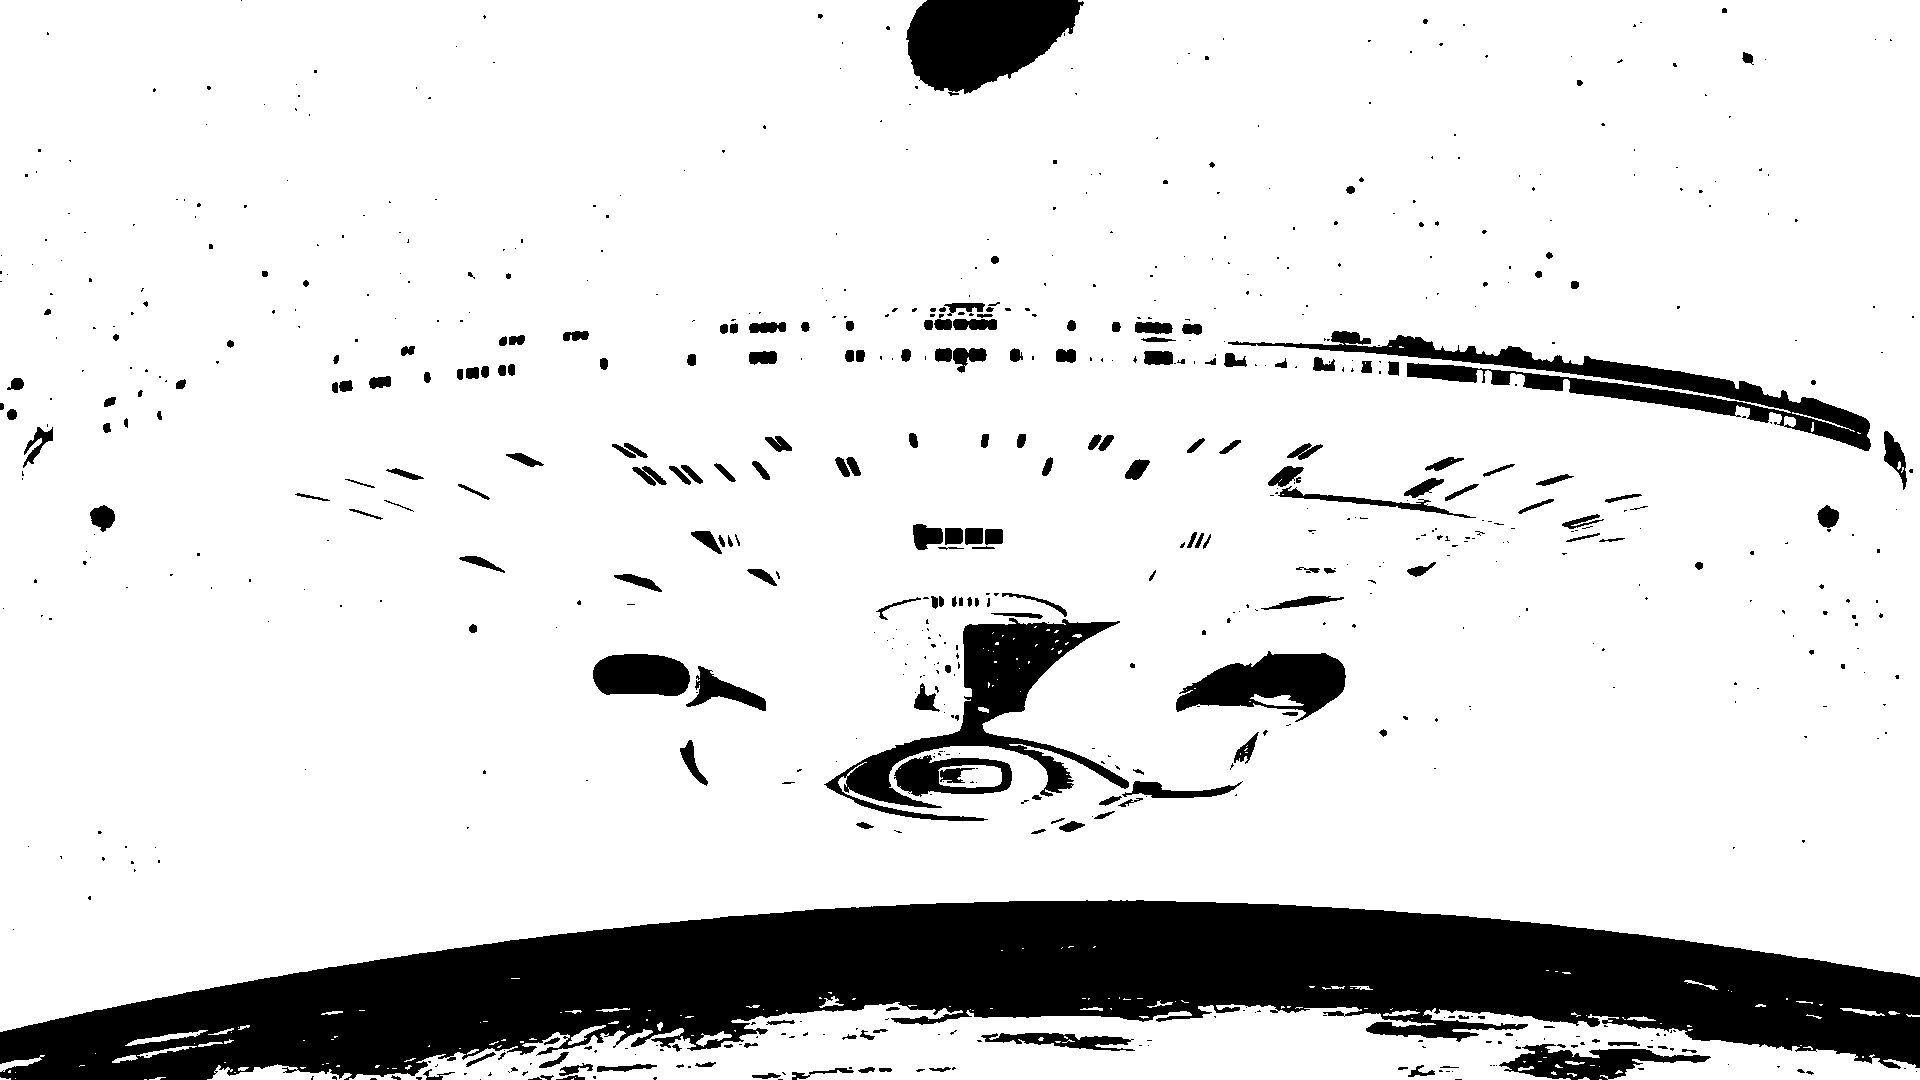
\includegraphics[width=0.97\linewidth]{_Figures/sample_3_bad_treshold.png}
    \caption{}
  \label{fig:tresh_bad_3}
\end{subfigure}

\begin{subfigure}{.3\textwidth}
  \centering
  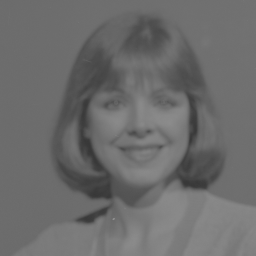
\includegraphics[width=0.97\linewidth]{_Figures/sample_4.png}
  \caption{}
  \label{fig:tresh_raw_4}
\end{subfigure}%
\begin{subfigure}{.3\textwidth}
  \centering
  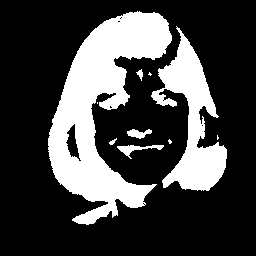
\includegraphics[width=0.97\linewidth]{_Figures/sample_4_good_treshold.png}
  \caption{}
  \label{fig:tresh_good_4}
\end{subfigure}%
\begin{subfigure}{.3\textwidth}
  \centering
  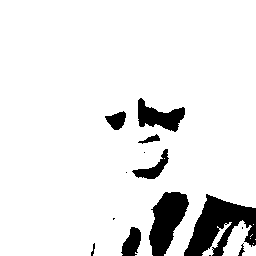
\includegraphics[width=0.97\linewidth]{_Figures/sample_4_bad_tresholding.png}
    \caption{}
  \label{fig:tresh_bad_4}
\end{subfigure}

\caption{Results for tresholding using experimental data.}
\label{fig:results_tresh}
\end{figure}

%
% HISTOGRAM
%
\subsection{Histogram Normalization Results}
Figure \ref{fig:histogram_results} represent results obtained by stretching histogram of test images. First column represents raw images (\ref{fig:raw_hist_1}, \ref{fig:raw_hist_2}, \ref{fig:raw_hist_3}, \ref{fig:raw_hist_4}), next one corresponds to images with average approach (\ref{fig:average_hist_1}, \ref{fig:average_hist_2}, \ref{fig:average_hist_3}, \ref{fig:average_hist_4})and the last one (\ref{fig:per_hist_1}, \ref{fig:per_hist_2}, \ref{fig:per_hist_3}, \ref{fig:per_hist_4}) per channel approach (as described in \ref{definitions})

As one can easily see, the process does not affect most of the pictures. In higher resolution it can be see that colors of figure \ref{fig:average_hist_1} are somehow more pleasant to the eye and quality of \ref{fig:raw_hist_4} has been drastically changed on \ref{fig:average_hist_4} and \ref{fig:per_hist_4}. On other two experimental data, no change has been observed.


\begin{figure}[h]
\centering
\begin{subfigure}{.3\textwidth}
  \centering
  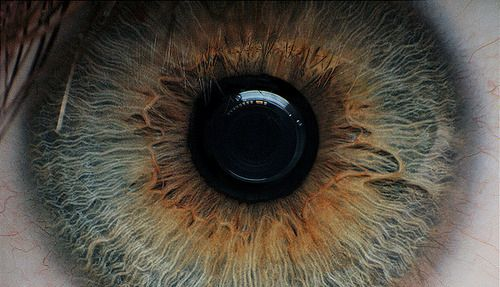
\includegraphics[width=0.97\linewidth]{_Figures/sample_1.jpg}
  \caption{}
  \label{fig:raw_hist_1}
\end{subfigure}%
\begin{subfigure}{.3\textwidth}
  \centering
  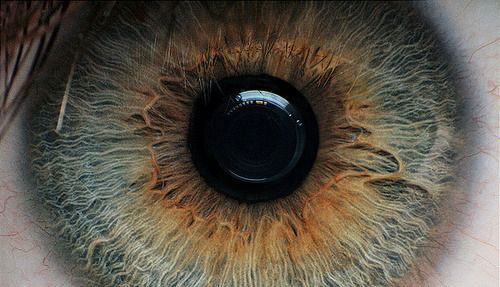
\includegraphics[width=0.97\linewidth]{_Figures/sample_1_normalization_average.png}
  \caption{}
  \label{fig:average_hist_1}
\end{subfigure}
\begin{subfigure}{.3\textwidth}
  \centering
  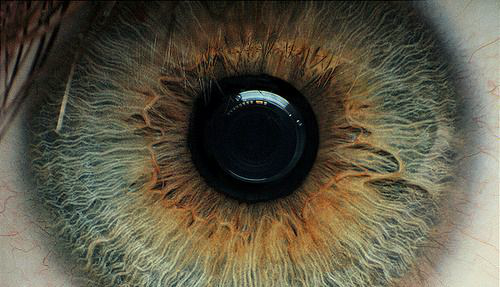
\includegraphics[width=0.97\linewidth]{_Figures/sample_1_normalization_per_channel.png}
  \caption{}
    \label{fig:per_hist_1}
\end{subfigure}%

\begin{subfigure}{.3\textwidth}
  \centering
  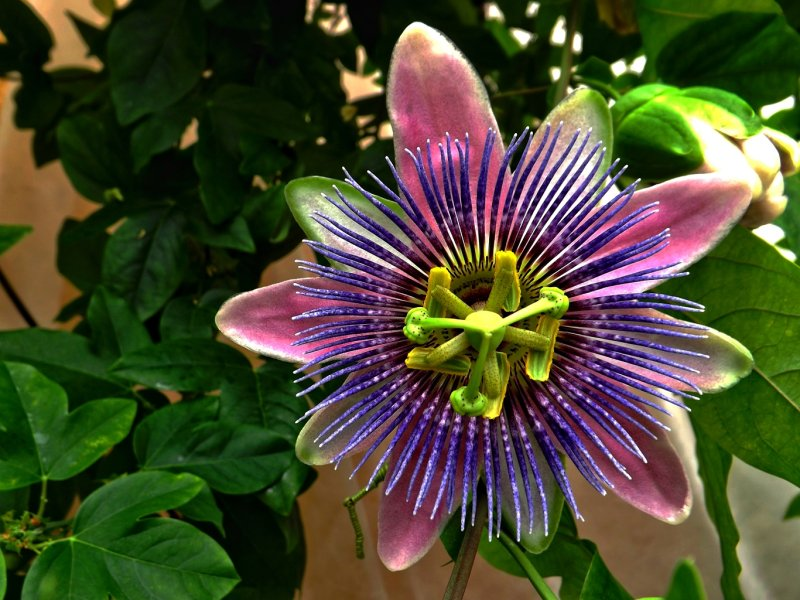
\includegraphics[width=0.97\linewidth]{_Figures/sample_2.jpg}
  \caption{}
  \label{fig:raw_hist_2}
\end{subfigure}%
\begin{subfigure}{.3\textwidth}
  \centering
  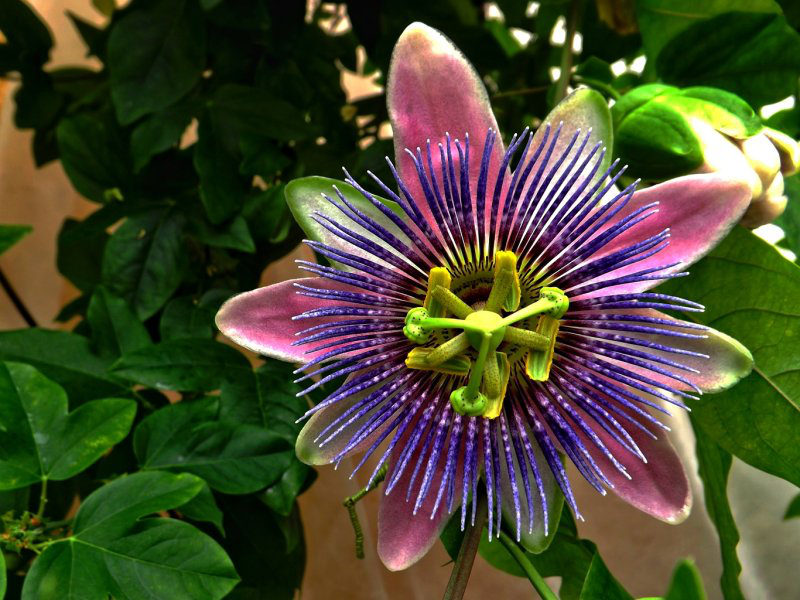
\includegraphics[width=0.97\linewidth]{_Figures/sample_2_normalization_average.png}
    \caption{}
      \label{fig:average_hist_2}
\end{subfigure}
\begin{subfigure}{.3\textwidth}
  \centering
  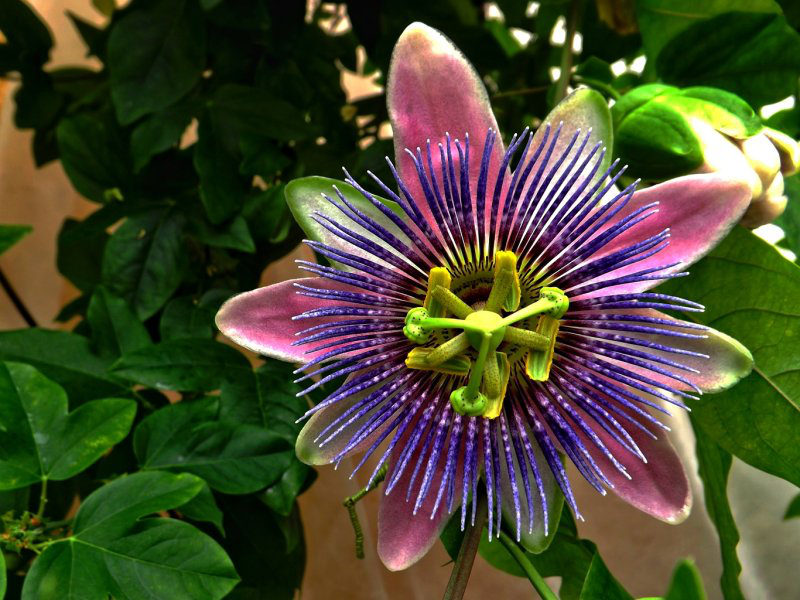
\includegraphics[width=0.97\linewidth]{_Figures/sample_2_normalization_per_channel.png}
    \caption{}
        \label{fig:per_hist_2}
\end{subfigure}


\begin{subfigure}{.3\textwidth}
  \centering
  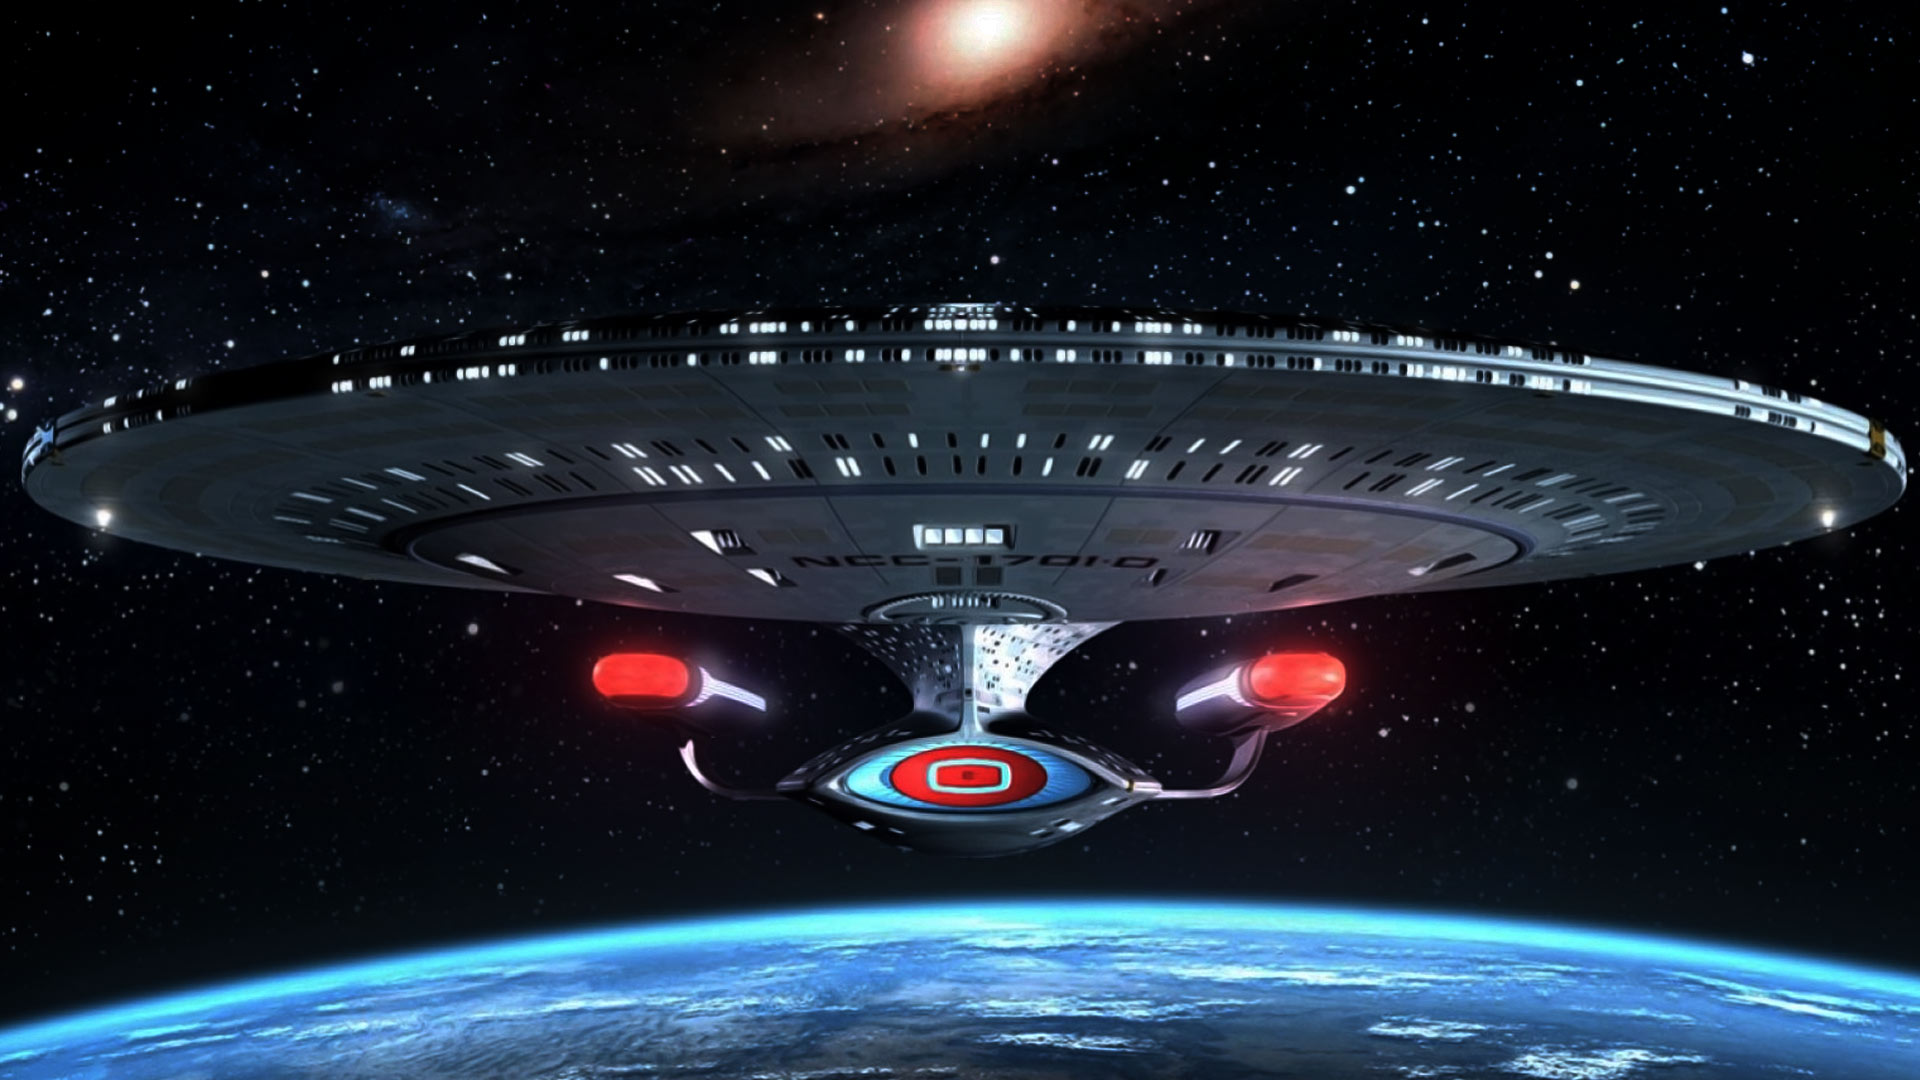
\includegraphics[width=0.97\linewidth]{_Figures/sample_3.jpg}
  \caption{}
  \label{fig:raw_hist_3}
\end{subfigure}%
\begin{subfigure}{.3\textwidth}
  \centering
  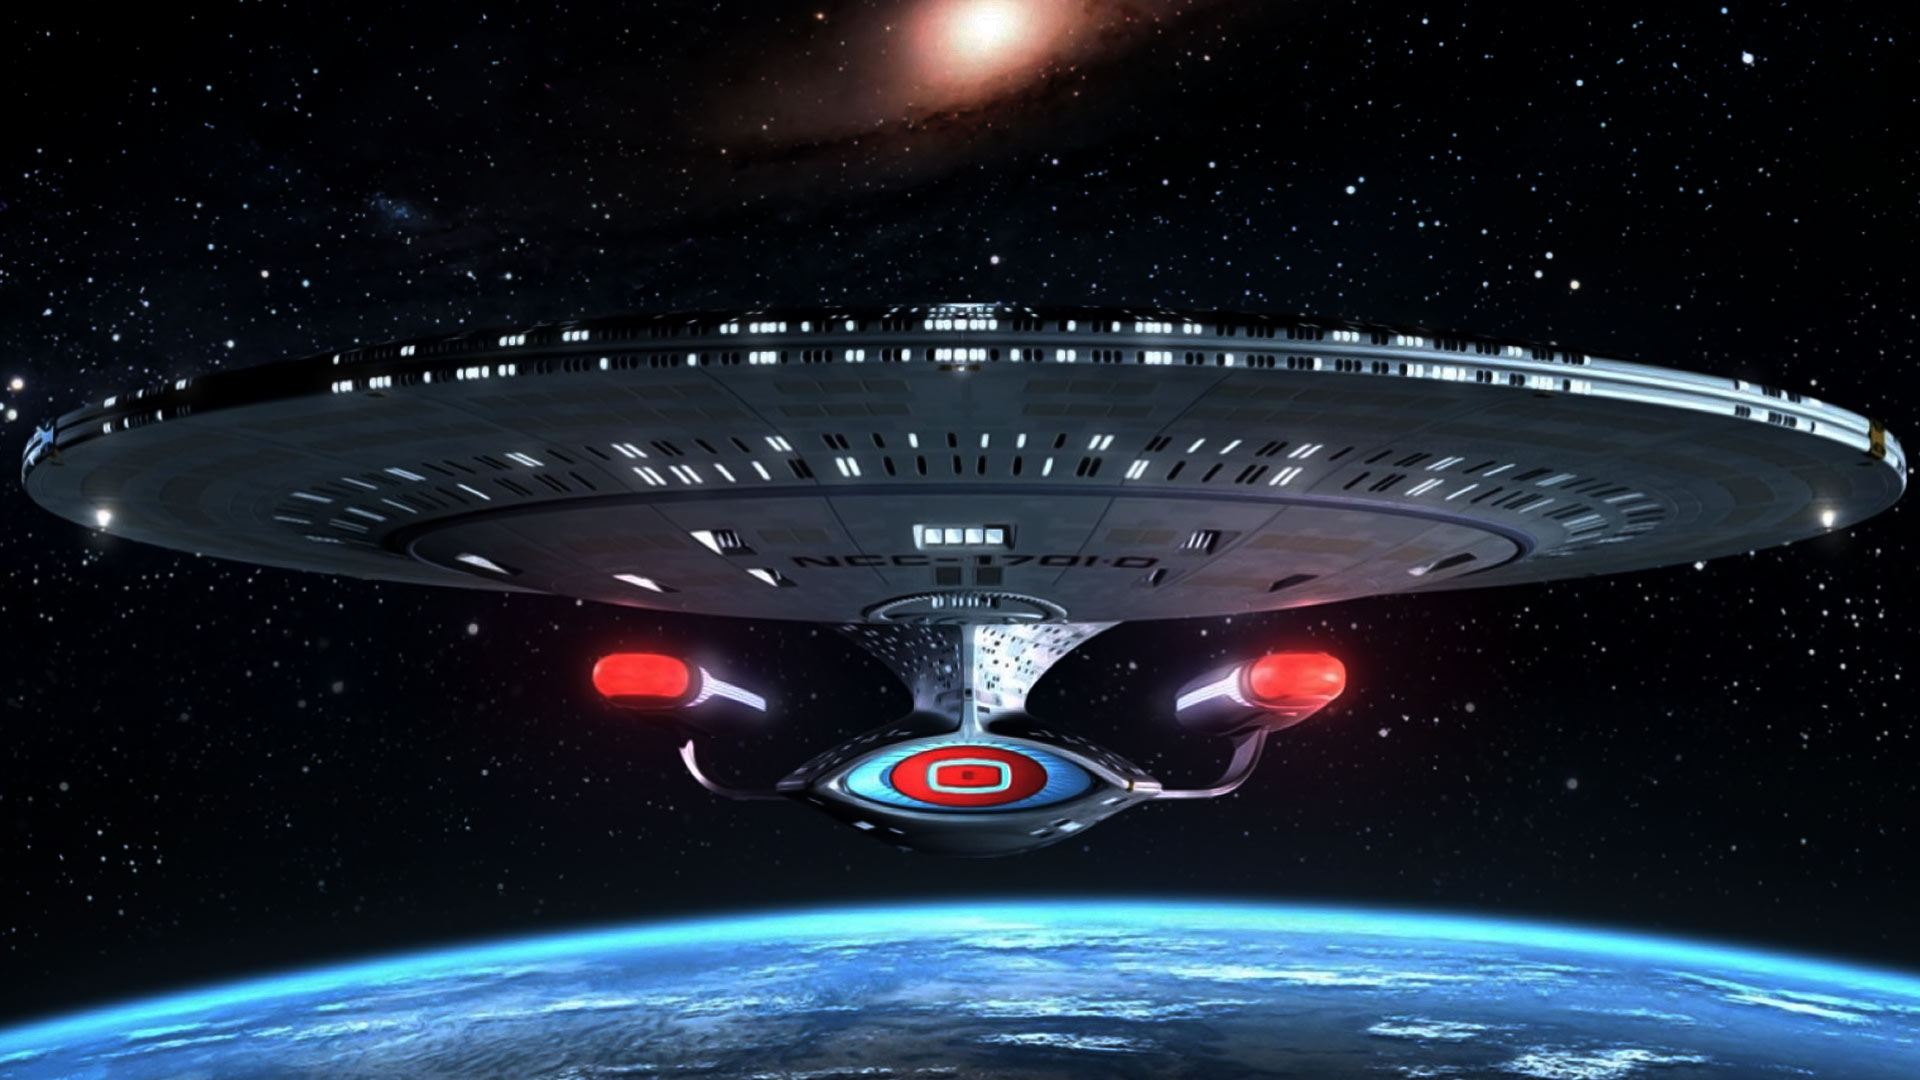
\includegraphics[width=0.97\linewidth]{_Figures/sample_3_normalization_average.png}
    \caption{}
      \label{fig:average_hist_3}
\end{subfigure}
\begin{subfigure}{.3\textwidth}
  \centering
  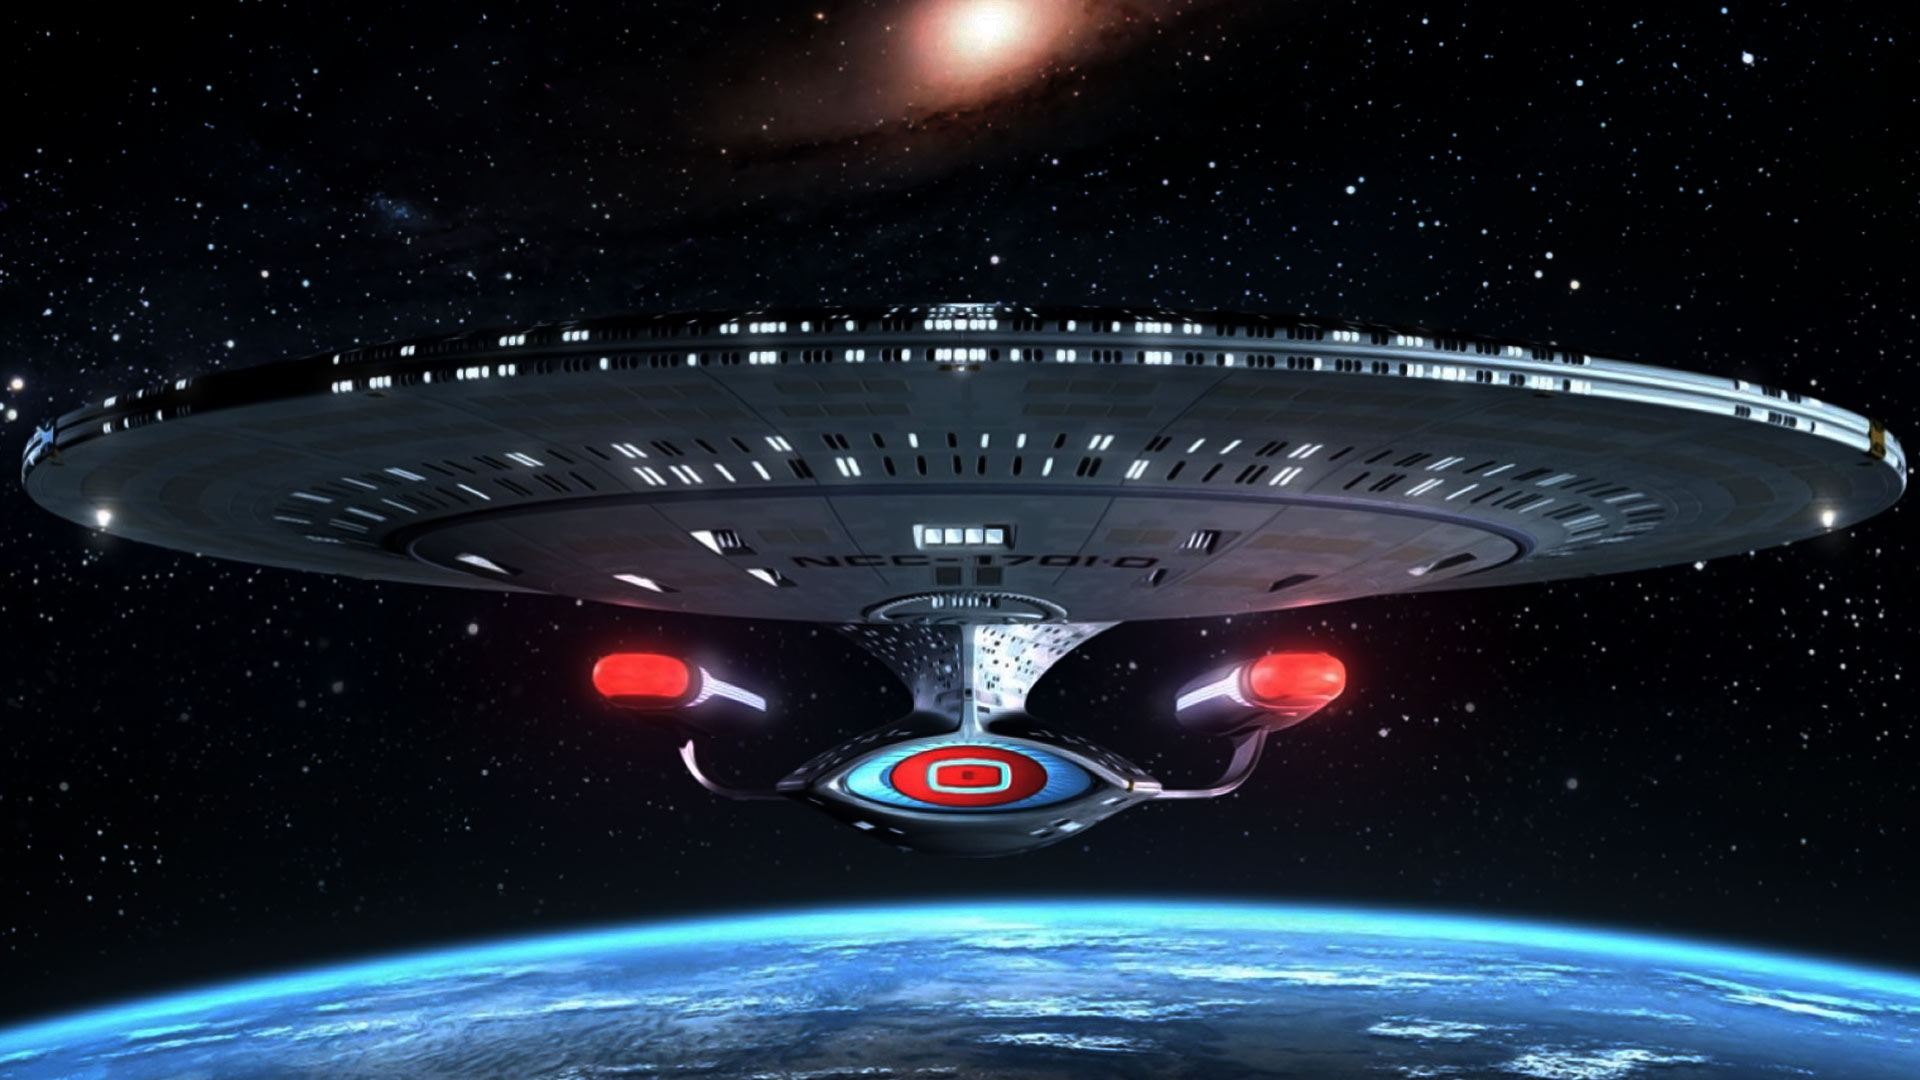
\includegraphics[width=0.97\linewidth]{_Figures/sample_3_normalization_per_channel.png}
    \caption{}
        \label{fig:per_hist_3}
\end{subfigure}

\begin{subfigure}{.3\textwidth}
  \centering
  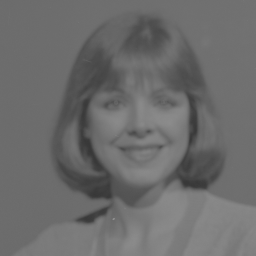
\includegraphics[width=0.97\linewidth]{_Figures/sample_4.png}
  \caption{}
   \label{fig:raw_hist_4}
\end{subfigure}%
\begin{subfigure}{.3\textwidth}
  \centering
  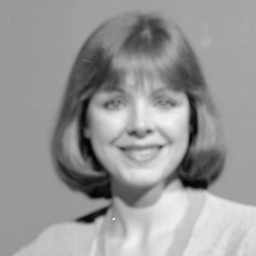
\includegraphics[width=0.97\linewidth]{_Figures/sample_4_normalization_average.png}
    \caption{}
      \label{fig:average_hist_4}
\end{subfigure}
\begin{subfigure}{.3\textwidth}
  \centering
  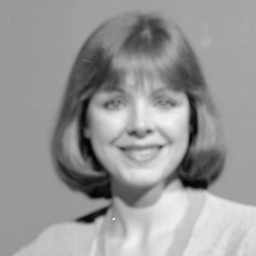
\includegraphics[width=0.97\linewidth]{_Figures/sample_4_normalization_per_channel.png}
    \caption{}
        \label{fig:per_hist_4}
\end{subfigure}


\caption{Results for histogram normalization of experimental data. }
\label{fig:histogram_results}
\end{figure}

%
% BRIGTHNESS
%
\subsection{Brightness Manipulation Results}
All pictures are acting rather the same - they have more and more light in process of adding brightness factor. All images were exposed to the same brightness level i.e \ref{fig:brigth_low_1}, \ref{fig:brigth_low_2}, \ref{fig:brigth_low_3}, \ref{fig:brigth_low_4} are at level 86 and \ref{fig:brigth_high_1}, \ref{fig:brigth_high_2}, \ref{fig:brigth_high_3}, \ref{fig:brigth_high_4} at level 186. From experimental data we see that only \ref{fig:brigth_high_4} is somehow all lost - it may be caused by the fact that it is in grayscale.

\begin{figure}[h]
\centering
\begin{subfigure}{.3\textwidth}
  \centering
  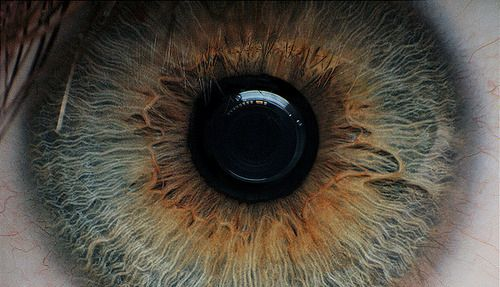
\includegraphics[width=0.97\linewidth]{_Figures/sample_1.jpg}
  \caption{}
  \label{fig:brigth_raw_1}
\end{subfigure}%
\begin{subfigure}{.3\textwidth}
  \centering
  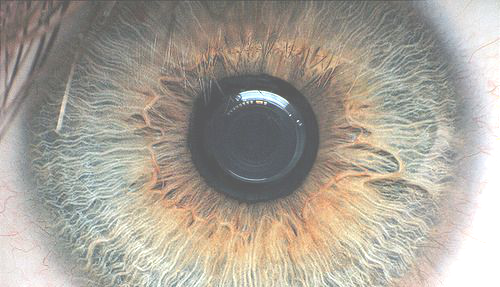
\includegraphics[width=0.97\linewidth]{_Figures/sample_1_brightness_low.png}
  \caption{}
  \label{fig:brigth_low_1}
\end{subfigure}
\begin{subfigure}{.3\textwidth}
  \centering
  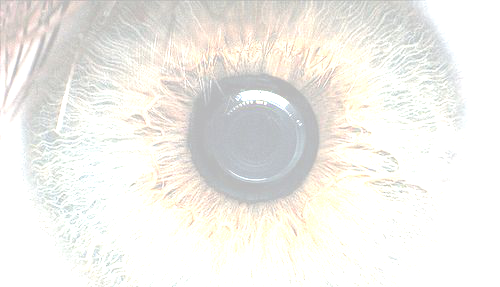
\includegraphics[width=0.97\linewidth]{_Figures/sample_1_brightness_high.png}
  \caption{}
    \label{fig:brigth_high_1}
\end{subfigure}%

\begin{subfigure}{.3\textwidth}
  \centering
  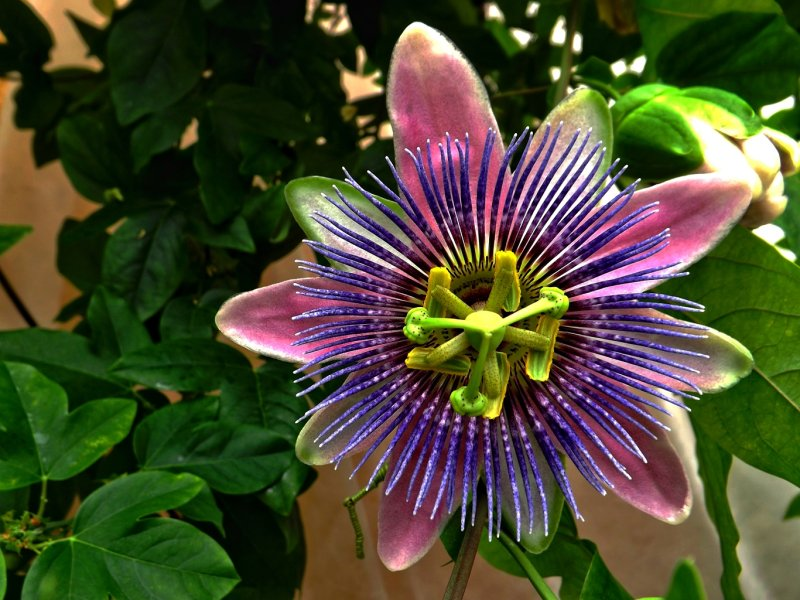
\includegraphics[width=0.97\linewidth]{_Figures/sample_2.jpg}
  \caption{}
  \label{fig:brigth_raw_2}
\end{subfigure}%
\begin{subfigure}{.3\textwidth}
  \centering
  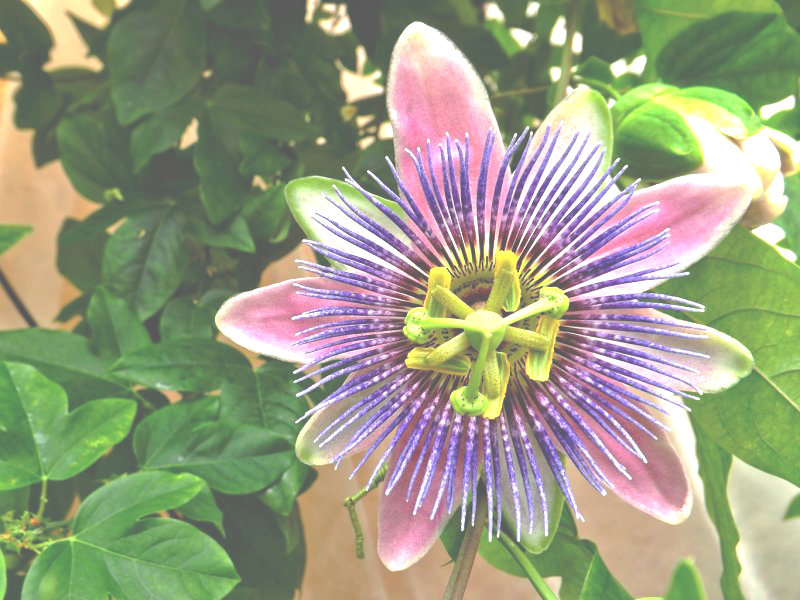
\includegraphics[width=0.97\linewidth]{_Figures/sample_2_brigthness_low.png}
    \caption{}
      \label{fig:brigth_low_2}
\end{subfigure}
\begin{subfigure}{.3\textwidth}
  \centering
  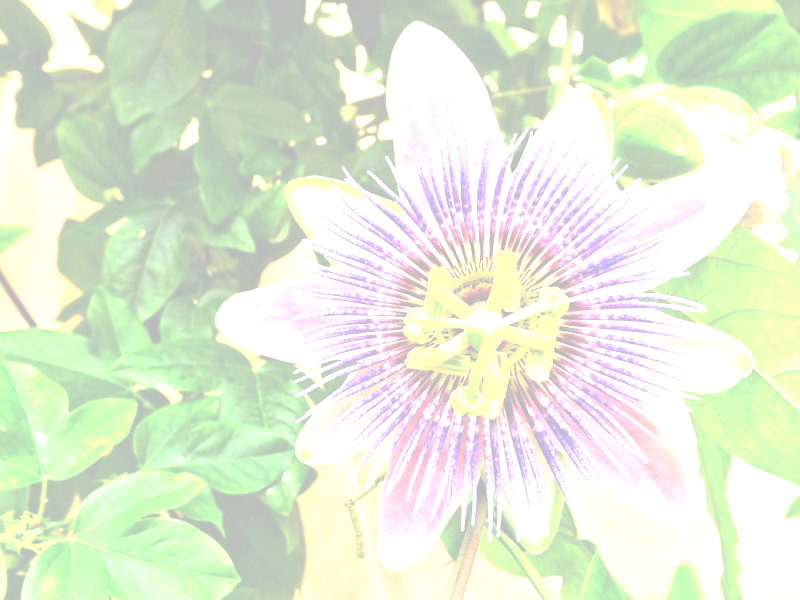
\includegraphics[width=0.97\linewidth]{_Figures/sample_2_brigthness_high.png}
    \caption{}
        \label{fig:brigth_high_2}
\end{subfigure}


\begin{subfigure}{.3\textwidth}
  \centering
  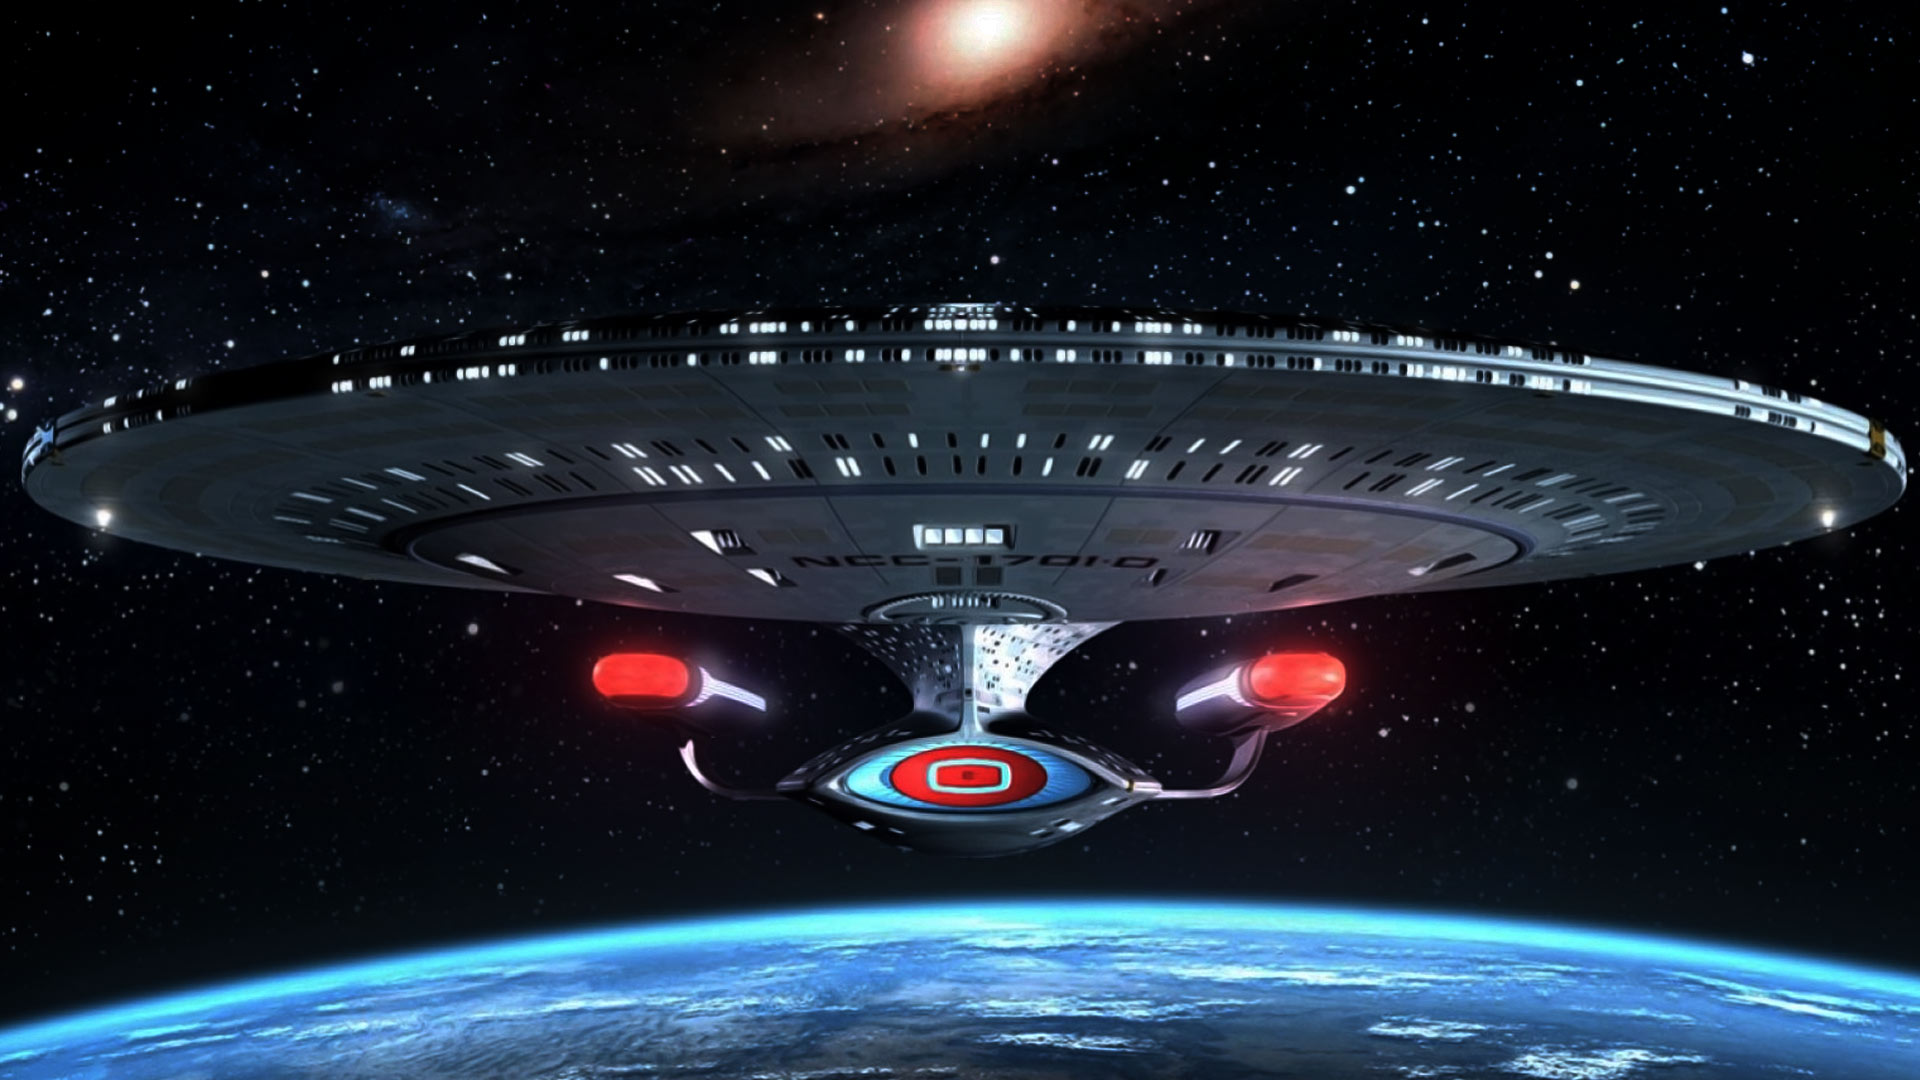
\includegraphics[width=0.97\linewidth]{_Figures/sample_3.jpg}
  \caption{}
  \label{fig:brigth_raw_3}
\end{subfigure}%
\begin{subfigure}{.3\textwidth}
  \centering
  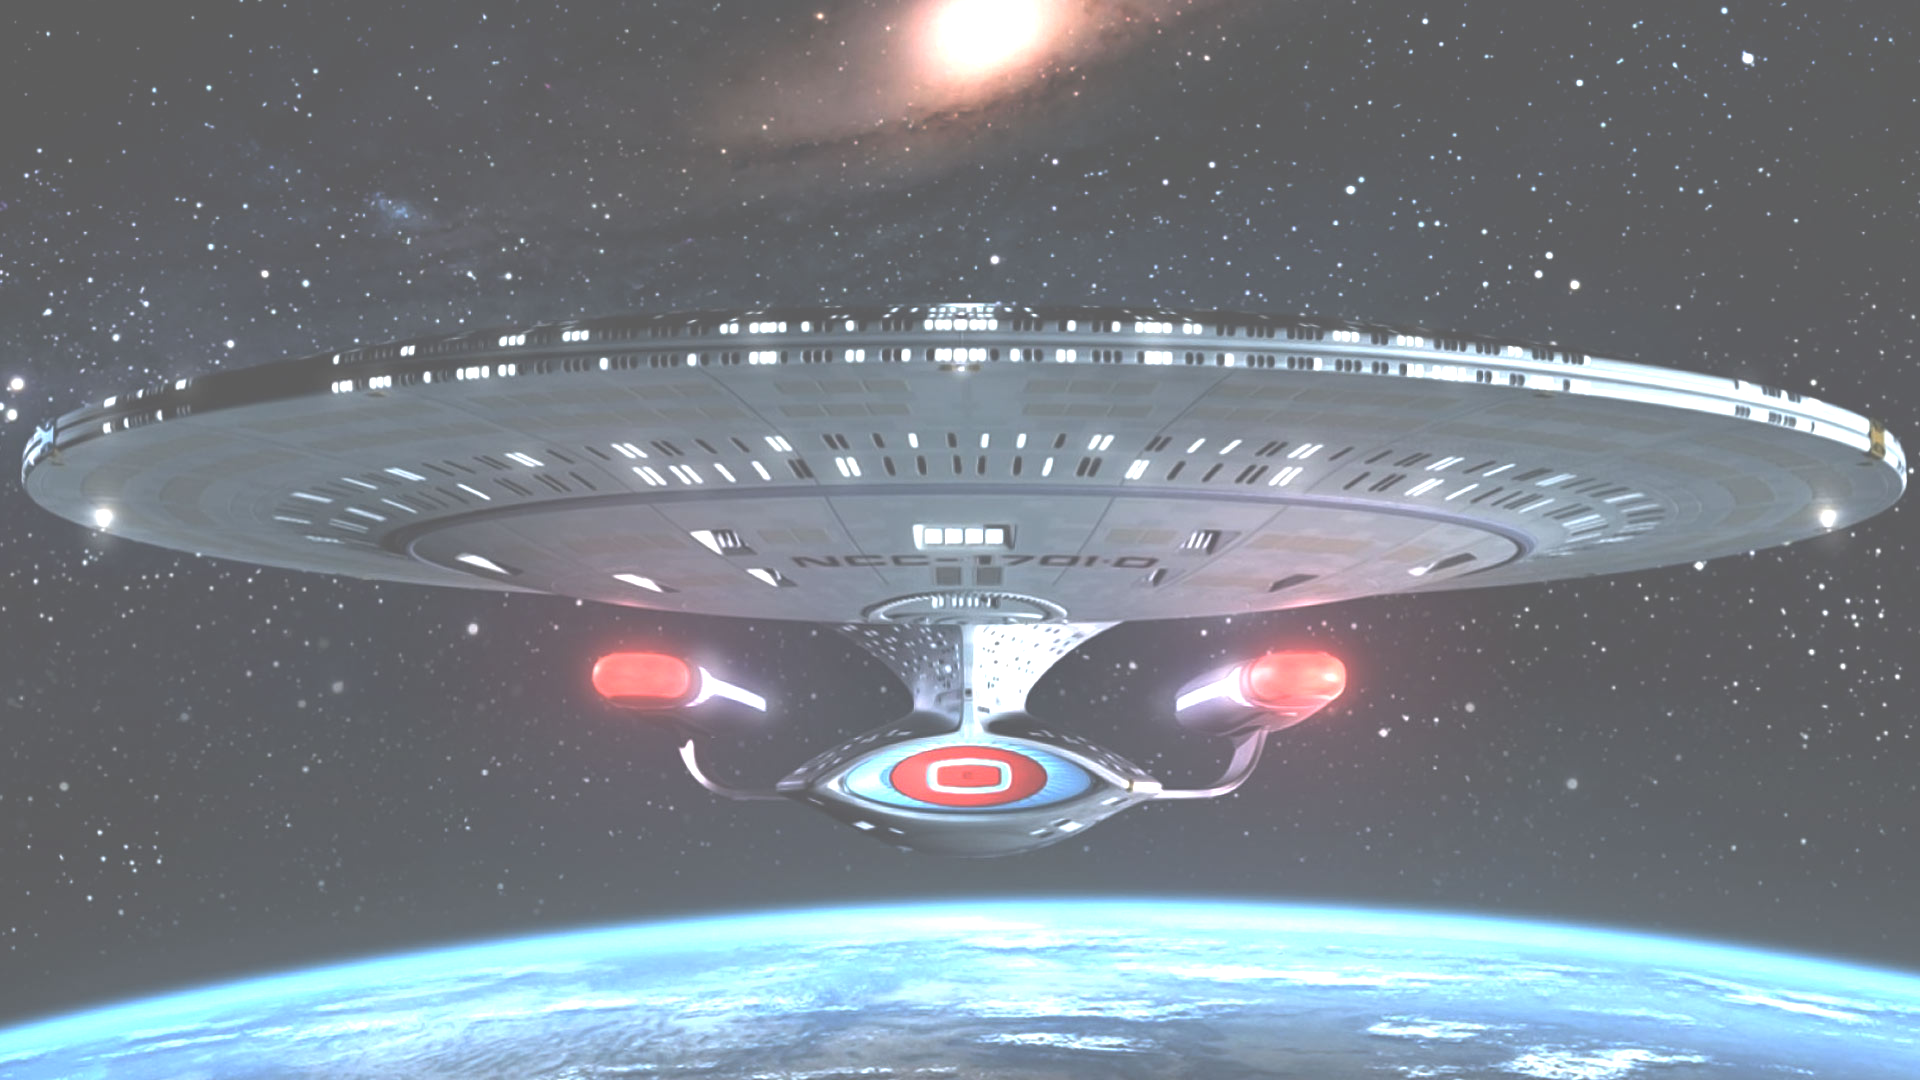
\includegraphics[width=0.97\linewidth]{_Figures/sample_3_brigthness_low.png}
    \caption{}
      \label{fig:brigth_low_3}
\end{subfigure}
\begin{subfigure}{.3\textwidth}
  \centering
  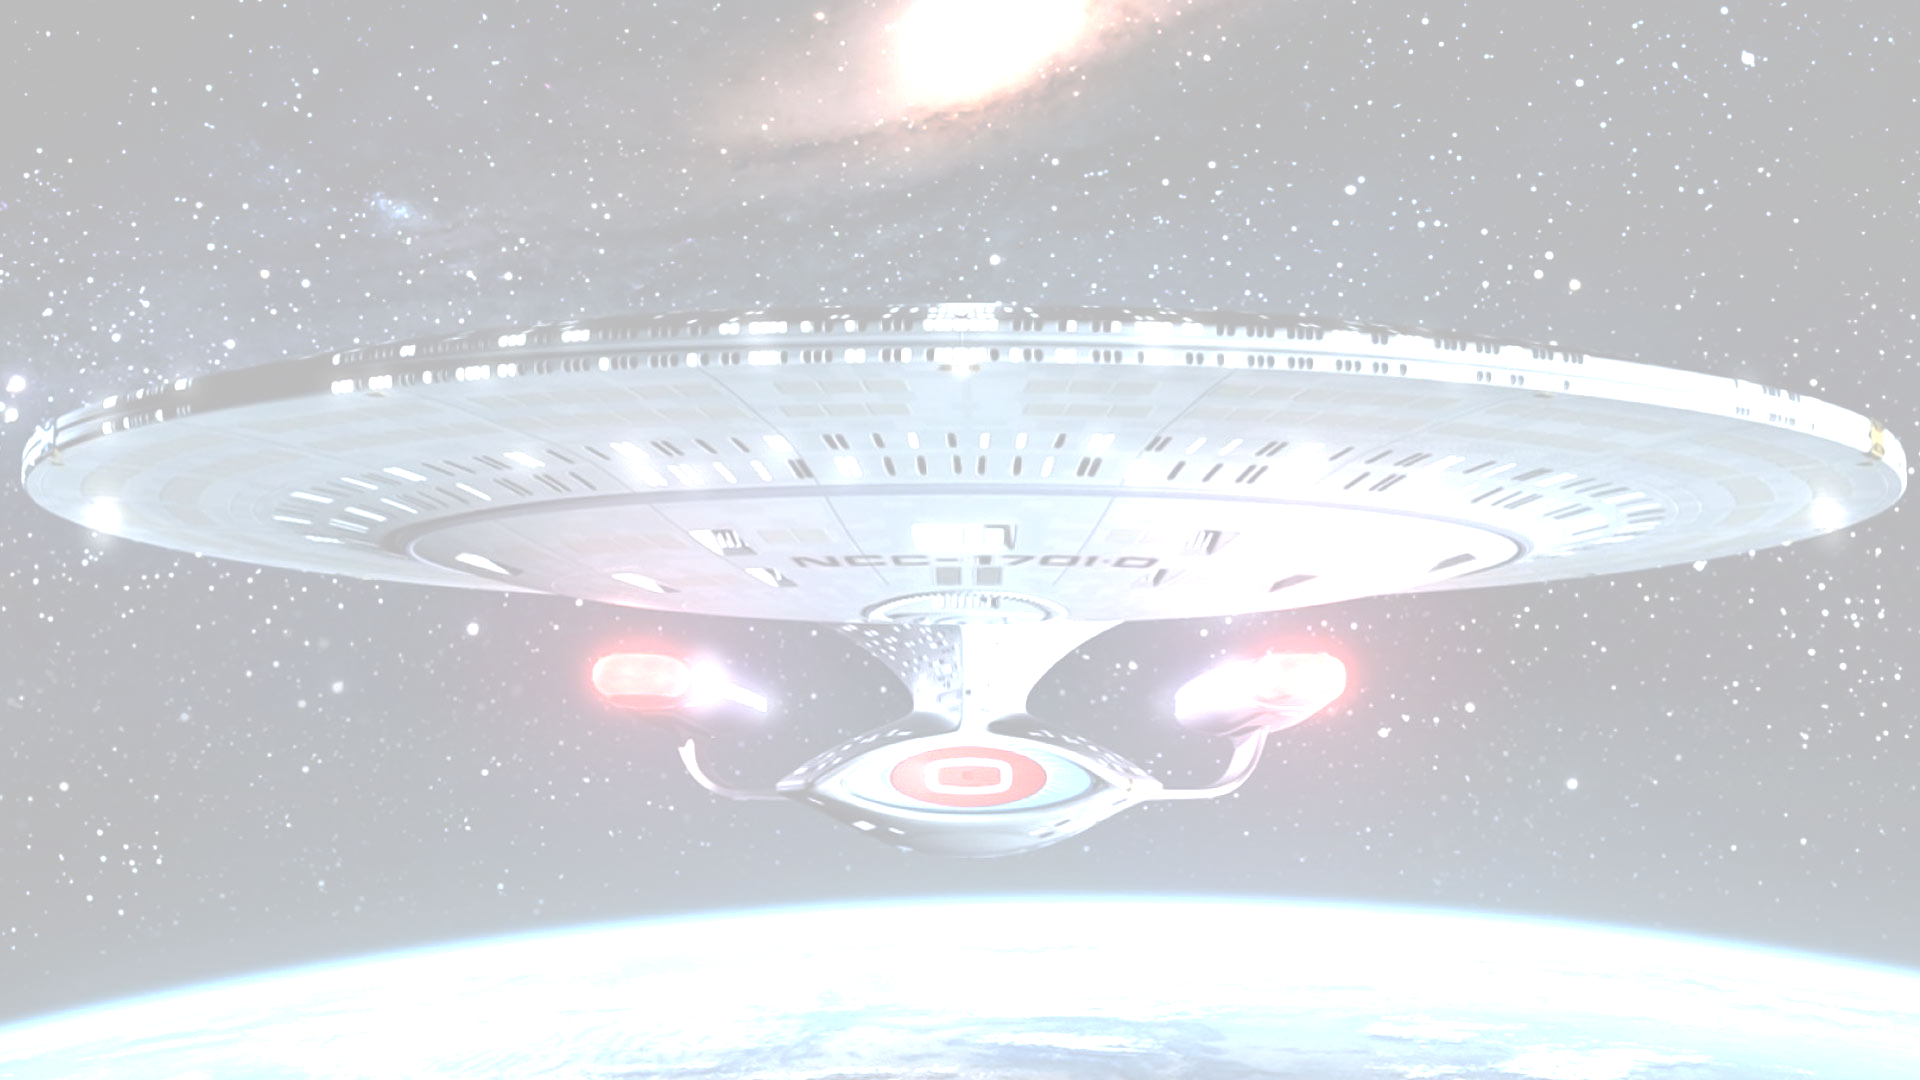
\includegraphics[width=0.97\linewidth]{_Figures/sample_3_brigthness_high.png}
    \caption{}
        \label{fig:brigth_high_3}
\end{subfigure}

\begin{subfigure}{.3\textwidth}
  \centering
  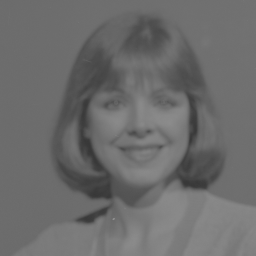
\includegraphics[width=0.97\linewidth]{_Figures/sample_4.png}
  \caption{}
   \label{fig:brigth_raw_4}
\end{subfigure}%
\begin{subfigure}{.3\textwidth}
  \centering
  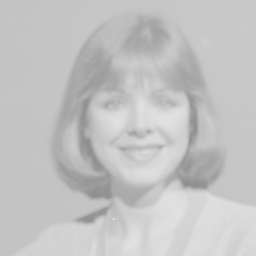
\includegraphics[width=0.97\linewidth]{_Figures/sample_4_brigthness_low.png}
    \caption{}
      \label{fig:brigth_low_4}
\end{subfigure}
\begin{subfigure}{.3\textwidth}
  \centering
  
\includegraphics[width=0.97\linewidth]{_Figures/sample_4_brigthness_high.png}
    \caption{}
        \label{fig:brigth_high_4}
\end{subfigure}


\caption{Results for brightness manipulation of experimental data. }
\label{fig:brigthness_results}
\end{figure}

To shortly sum up - all pictures were acting as assumed. Although histogram normalization required more work to implement, almost nothing can be seen on the experimental images. It may be caused by bad selection process - maybe \ref{fig:sample_2} and \ref{fig:sample_3} were already normalized? We will never know.
%----------------------------------------------------------------------------------------
%	BIBLIOGRAPHY
%----------------------------------------------------------------------------------------
\newpage

\begin{thebibliography}{1}
	\bibitem{tresholding_def} \url{https://www.wordnik.com/words/thresholding}
	\bibitem{image_histogram_def} \url{https://svi.nl/ImageHistogram}
	\bibitem{histogram_normalization_def} \url{https://en.wikipedia.org/wiki/Normalization_(image_processing)}
	\bibitem{brightness_def1} \url{http://olympusmicro.com/primer/java/olympusmicd/digitalimaging/contrast/index.html}
\end{thebibliography}

%----------------------------------------------------------------------------------------


\end{document}